\chapter{Hero Run Data Analysis} 
\label{chapter5}

The work described here details the capstone efforts of this PhD dissertation, aiming to analyze this massive pool of data and extract meaningful chemical insights.
The fully scaled version of the Early Earth simulation, a system of 22.8 million atoms referred to as the HiPerGator Hero Run, represents the most extensive reactive molecular dynamics simulation ever conducted with a machine-learned interatomic potential.
This ambitious project was undertaken as a collaboration between the HiPerGator research computing team, NVIDIA, and the Roitberg group, testing the limits of NVIDIA GPU technology on the HiPerGator supercomputer with state-of-the-art neural network potentials to model prebiotic chemistry on an unprecedented scale.
The first analysis of the Hero Run trajectory data was conducted by Dr. Jinze Xue during the reservation of all 1,048 GPUs on HPG.
This initial scan was conducted by splitting each of the 44 trajectory files into 20 segments and distributing the analysis across 880 GPUs.
From this first search, over 5.5 million named molecules from the PubChem dataset (Table \ref{tbl:molfind_targets}) were identified; the number of appearances of each molecule matching a structure in the PubChem dataset with this initial scan are presented in Figure \ref{fig:initial_scan}.

\begin{figure}[!h]
    \centering
    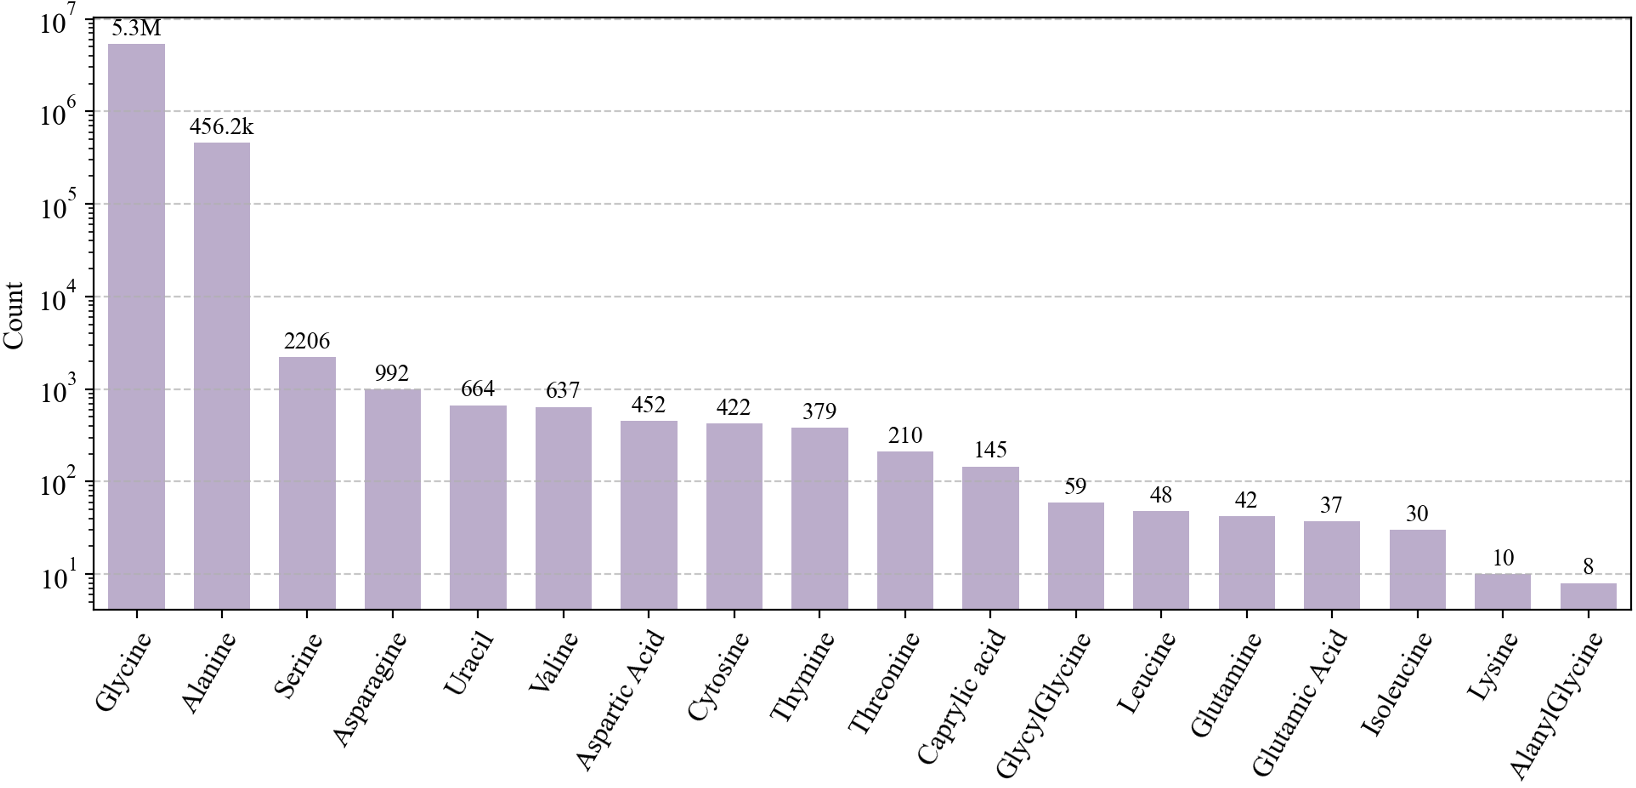
\includegraphics[width=1\linewidth]{Images/early_earth/updated_original_counts.png}
    \caption[Molecules identified in the initial search]{Named molecules identified in the initial search through the trajectory data ($N=5,789,046$). }
    \label{fig:initial_scan}
\end{figure}

From the first scan, we saw that most molecules (within the limited subset of chemical space in the PubChem dataset) synthesized throughout this simulation are glycine, though we see the formation of 14 different amino acids.
We then shifted the focus of this project toward expanding the PubChem dataset to a much larger set of molecules of interest.
The next sections detail the strategies developed to process, analyze, and extract meaningful insights from this massive pool of raw trajectory data, including custom GPU-accelerated implementations for graph-based molecular identification, filtering, and clustering techniques.
The scripts and relevant code used in performing this analysis are tracked and stored on the GitHub page \href{https://github.com/nterrel/early_earth_analysis}{nterrel/early\_earth\_analysis}.

\section{Overhauling the Molfind Analysis Tool}
\label{sec:molfind_updates}

The \verb|molfind| program works very well for highly-distributed analysis across hundreds of GPUs.
A major limitation of this approach is that hundreds of GPUs are seldom available for simulatneous use in academic research.
With an allocation of 16 GPUs on HiPerGator, the same analysis that takes only 6 hours across 880 GPUs would take 13.75 days---assuming one can run constantly with no downtime, which is a major assumption on a supercomputer with an average of 500 GPUs in use at any time \cite{hpg_metrics}.
Being limited to a small number of GPUs, we must look for ways to increase computational efficiency at every stage of the data processing pipeline. 

\subsection{Loading Simulation Data into Memory}
\label{subsec:top_loader}

The first obstacle encountered in trying to analyze this data on a smaller scale was the time required to load a single frame from the simulation into memory. 
Splitting the trajectory into smaller chunks requires a clever approach to avoid overloading system memory by loading an entire 2 TB file. 
The \verb|iterload| function within \verb|MDTraj| \cite{mdtraj} works well to separate certain frames from the trajectory, provided the frames of interest are known.
A single-frame of the trajectory stored in \verb|dcd| format occupies 274 megabytes of disk space.
In order to load a trajectory into memory, \verb|MDTraj| requires two inputs: a trajectory file, and a topology file.

Traditionally in molecular dynamics, a topology file lists the atom indices, identities, and what molecule those atoms reside in.
In reactive MD, we have a constantly changing topology, meaning that no bonds are fixed.
We still, however, need to set a topology file to load the trajectory data into memory.
In the initial version of \verb|molfind|, a \verb|pdb| format topology is used. 
Loading this as the system topology (atom indices to identify coordinates stored in \verb|dcd| format) took an average of 7 minutes and 48 seconds, without performing any analysis.
To improve the loading time, we converted individual frames into \verb|HDF5| format with \verb|MDTraj.convert|, and using the \verb|MDTraj.load| function to load this combined trajectory and topology we see a speedup of $\sim5.4\text{x}$ to an average loading time of 86.2 seconds.
As this was still the rate-limiting step in analyzing a single frame of the simulation trajectory with \verb|molfind|, and given that \verb|MDTraj| is an open-source software, we looked for speedups in the \verb|mdtraj.load().topology| method to streamline the loading of a topology stored in \verb|HDF5| format.
The custom topology loader function (\verb|load_topology|) used for opening an \verb|HDF5| file as a \verb|Topology| object is provided in Appendix \ref{appendix:loader_function} and timings for the three methods of loading the simulation topology are provided in Table \ref{tbl:top_loader_timings}.

\begin{table}[h!]
\centering
\caption[Hero Run topology loading times]{Comparison of file size and loading times with MDTraj in PDB and HDF5 formats against the customized loader function.
}\label{tbl:top_loader_timings}
\begin{tabularx}{0.63\textwidth}{lrrr}  
\toprule
Loading method & File size & Time (s) & Speedup \\
\midrule
PDB via MDTraj & 1.8 GB & 467.8 & 1x \\
HDF5 via MDTraj & 1.3 GB & 86.2 & 5.43x \\
HDF5 via \verb|load_topology| & 1.3 GB & 36.0 & 13.0x \\
\bottomrule
\end{tabularx}
\end{table}

The next step was to extract from the simulation data the structures of molecules that match entries of the PubChem dataset. 
In the initial analysis, only atom indices of relevant molecules were saved, and with a more efficient approach to loading the system into memory, extracting the coordinates of these molecules became feasible on a limited allocation of computational resources.
Extracting coordinates from atom indices from a single frame is a slow process due to the time taken to load the system into memory; iterating over hundreds or thousands of frames is far faster.
Once the system topology is loaded, iterating over frames takes less than one second per loop.
The first target of a detailed analysis was alanine.
Inspection of the \textit{very first} alanine extracted showed that some structures identified as alanine molecules were actually just constitutional isomers rather than exact matches.
This is due to the definition of isomorphism between two graphs in \verb|NetworkX| \cite{networkx}. 

\subsection{Categorical Graph Matching}
\label{subsec:molfind_graphmatcher}

Figure \ref{fig:mismatched_alanine}(A) shows the first alanine detected at 0.1670 ns into the simulation.
Here, there is an extra hydrogen bonded on the amino group, and this structure lacks a carboxylic acid.
This structure was misidentified because the \verb|networkx.is_isomorphic()| function checks only for the existence of nodes and edges on two graphs that can be superimposed.
Without additional logic for matching the identities of nodes (elements) and edges (bonds), the graph comparison was blindly looking at the shape of two graphs to determine isomorphism. 
Figure \ref{fig:mismatched_alanine}(B) demonstrates how NetworkX was looking at a molecule where, without atom identities, one could be convinced that this is an alanine molecule.

\begin{flushleft}
\begin{multiFigure}
    \addFigure{0.5}{Images/early_earth/alanine.png}
    \addFigure{0.5}{Images/early_earth/alanine_shaded.png}
\captionof{figure}[Mismatched structure of alanine]{
(A) Structure misidentified as alanine and
(B) how NetworkX was interpreting this structure, which makes it appear to be an alanine molecule.}
\label{fig:mismatched_alanine}
\end{multiFigure}
\end{flushleft}

For each fragment graph with a formula matching an entry of the PubChem dataset, the nodes and edges were unlabeled.
This meant that a molecule with the correct stoichiometry but different connectivity could match a structure in the reference database.
Correcting this required implementing additional logic to determining graph isomorphism.
A categorical node-matching approach was taken, where each node in the target and reference graphs are given labels corresponding to their atom types, and the edges between these nodes are labeled with a sorted (alphabetized) list of the two elements participating in each bond.
The code used to implement this is provided in Appendix \ref{appendix:graph_matcher}, along with the implementation of this into the loop where we compare two reference graphs.
This requires additional processing for each graph, but the slow step in analyzing frames for molecules of interest lies in creating the fragment graphs in the first place, and this operation still occurs on the order of microseconds per molecule. 

Using a categorical node and edge matching strategy ensures that corresponding atoms and bonds must have the same chemical identity for the two subgraphs to be considered isomorphic. 
If the subgraph is determined to be isomorphic to a reference, \verb|molfind| then assigns the corresponding label (e.g., “alanine” or “glycine”) to the fragment. 
The analysis was conducted once more with the updated \verb|GraphMatcher|, removing the species that were overestimated in the original search due to misidentification. 
This adjustment led to an updated count of molecules matching a reference in the PubChem database, provided in Figure \ref{fig:graph_matching}, though the overestimation was much less severe than originally thought.

\begin{figure}[!h]
    \centering
    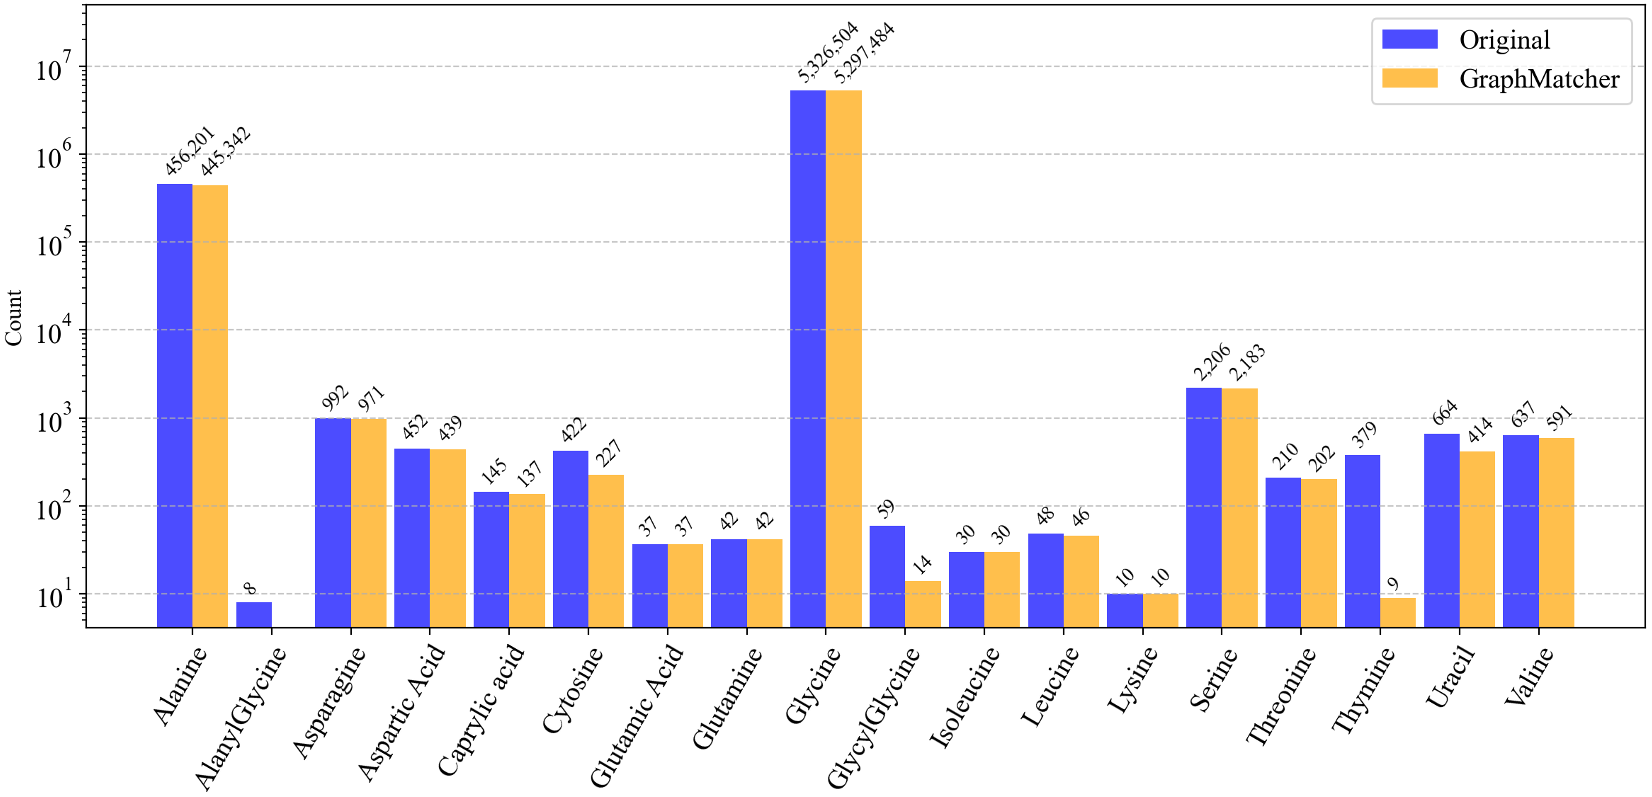
\includegraphics[width=1\linewidth]{Images/early_earth/updated_graphmatcher.png}
    \caption[Molecules identified incorrectly in the initial search]{Molecule counts before and after correcting the graph-matching algorithm.}
    \label{fig:graph_matching}
\end{figure}

Fortunately, the first alanine molecule detected in the simulation was not representative of a massive overestimation; the values from Figure \ref{fig:graph_matching} are provided in Table \ref{tbl:graphmatcher_counts}.

\begin{table}[h!]
\centering
\caption[Comparison of Isomorphism versus GraphMatcher identification]{Matching structures with NetworkX Isomorphism versus GraphMatcher.
}\label{tbl:graphmatcher_counts}
\begin{tabularx}{0.51\textwidth}{lrr}  
\toprule
Molecule & Isomorphism & GraphMatcher \\
\midrule
Alanine & 456,201 & 445,342\\
AlanylGlycine & 8 & 0 \\
Asparagine & 992 & 971 \\
Aspartic acid & 452 & 439 \\
Caprylic acid & 145 & 137 \\
Cytosine & 422 & 227 \\
Glutamic acid & 37 & 37 \\
Glutamine & 42 & 42 \\ 
Glycine & 5,326,504 & 5,297,484 \\
GlycylGlycine & 59 & 14 \\
Isoleucine & 30 & 30 \\
Leucine & 48 & 46 \\
Lysine & 10 & 10 \\
Serine & 2,206 & 2,183 \\
Threonine & 210 & 202 \\
Thymine & 379 & 9 \\
Uracil & 604 & 414 \\
Valine & 637 & 591 \\
Total & 5,789,046 & 5,748,178 \\
\bottomrule
\end{tabularx}
\end{table}

It is important to note that the majority of structures were correctly identified, though more than 40,000 structures were misidentified.
This was, unexpectedly, more common as molecular complexity increases.
In particular, identifying dipeptides and nitrogenous bases saw significant decreases in the count of ``true" matches.
Glycylglycine were misidentified in $\sim$76\% of cases, while every alanylglycine was misidentified every time.
Cytosine was misidentified $\sim$46\% of the time, and thymine was misidentified in 97.6\% of cases.
While this approach cuts down on the data extracted, rigorous assignment of node and edge attributes makes the GraphMatcher a powerful method for confirming the presence of specific molecules within highly complex molecular dynamics trajectories.


The next challenge was extracting molecules from this massive pool of data.
If we wanted to look at any specific structures, we need to open the trajectory and pull out the coordinates.
With the improved topology loader detailed in Subsection \ref{subsec:top_loader}, the coordinates of all identified molecules---excluding glycine, which made up $\sim$92\% of the molecules identified---were iteratively extracted by referencing a list of frame numbers and atom indices listed in the \verb|molfind| output \verb|df_molecule| (described in Subsection \ref{subsec:molfind}).
A few glycine molecules were extracted by hand, but storing all 5.3 million structures was a pointless exercise as a starting point.

The first target of a comprehensive review is alanine, of which the GraphMatcher identified a total of 445,342 structures. 
With the corrected graph-matching procedure in place, the identification of alanine molecules in the simulation is now more reliable, allowing for a detailed analysis of their structural properties. 
The extracted structures, however, had another complication: the coordinates were ordered arbitrarily based on the graph fragmentation protocol.
Even alanine molecules that persisted for several sequential frames had mismatched indices when the coordinates were saved, leading to strange behavior in visualization.
In order to align and visualize these structures, and compute structural properties, the atomic indices were remapped to a standard reference using a similar approach to the GraphMatcher described above.
Dihedral angles were measured across the atoms labeled in Figure \ref{fig:alanine_dih_labeled} to plot the conformational distribution shown in Figure \ref{fig:ala_dihedral}.

\begin{figure}[!ht]
    \centering
    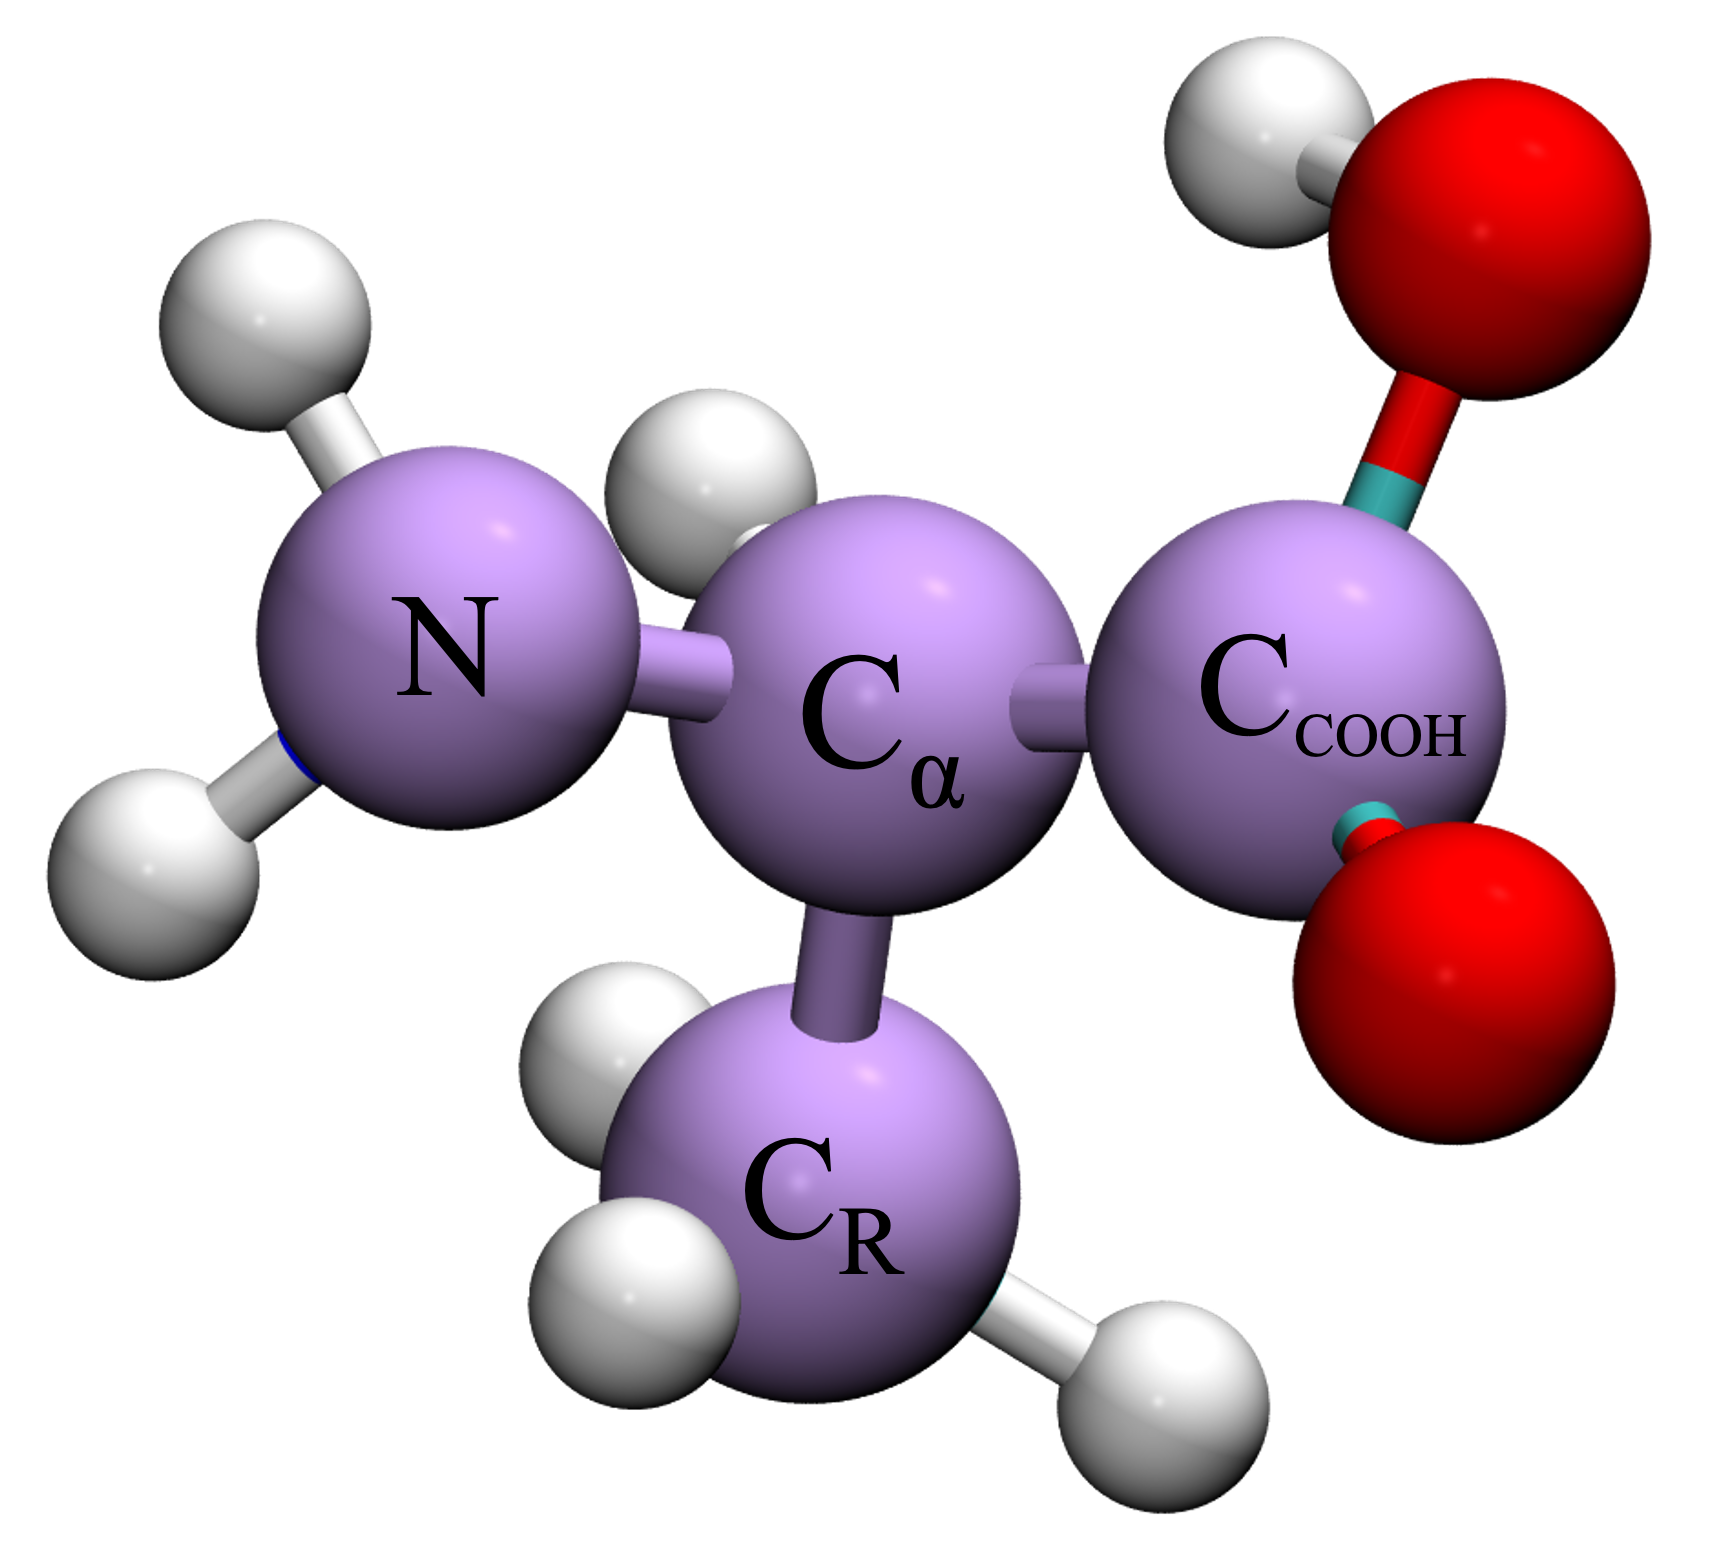
\includegraphics[width=0.5\linewidth]{Images/alanine_dihedral/dihedral_alanine.png}
    \caption[Atoms used in computing alanine dihedral angles]{Dihedral angles of extracted alanines were computed as the deviation of the R-group carbon ($\text{C}_\text{R}$) from the plane of the amino nitrogen (N), alpha carbon ($\text{C}_\alpha$), and the carboxyl carbon ($\text{C}_\text{COOH}$).}
    \label{fig:alanine_dih_labeled}
\end{figure}

\begin{figure}[!ht]
    \centering
    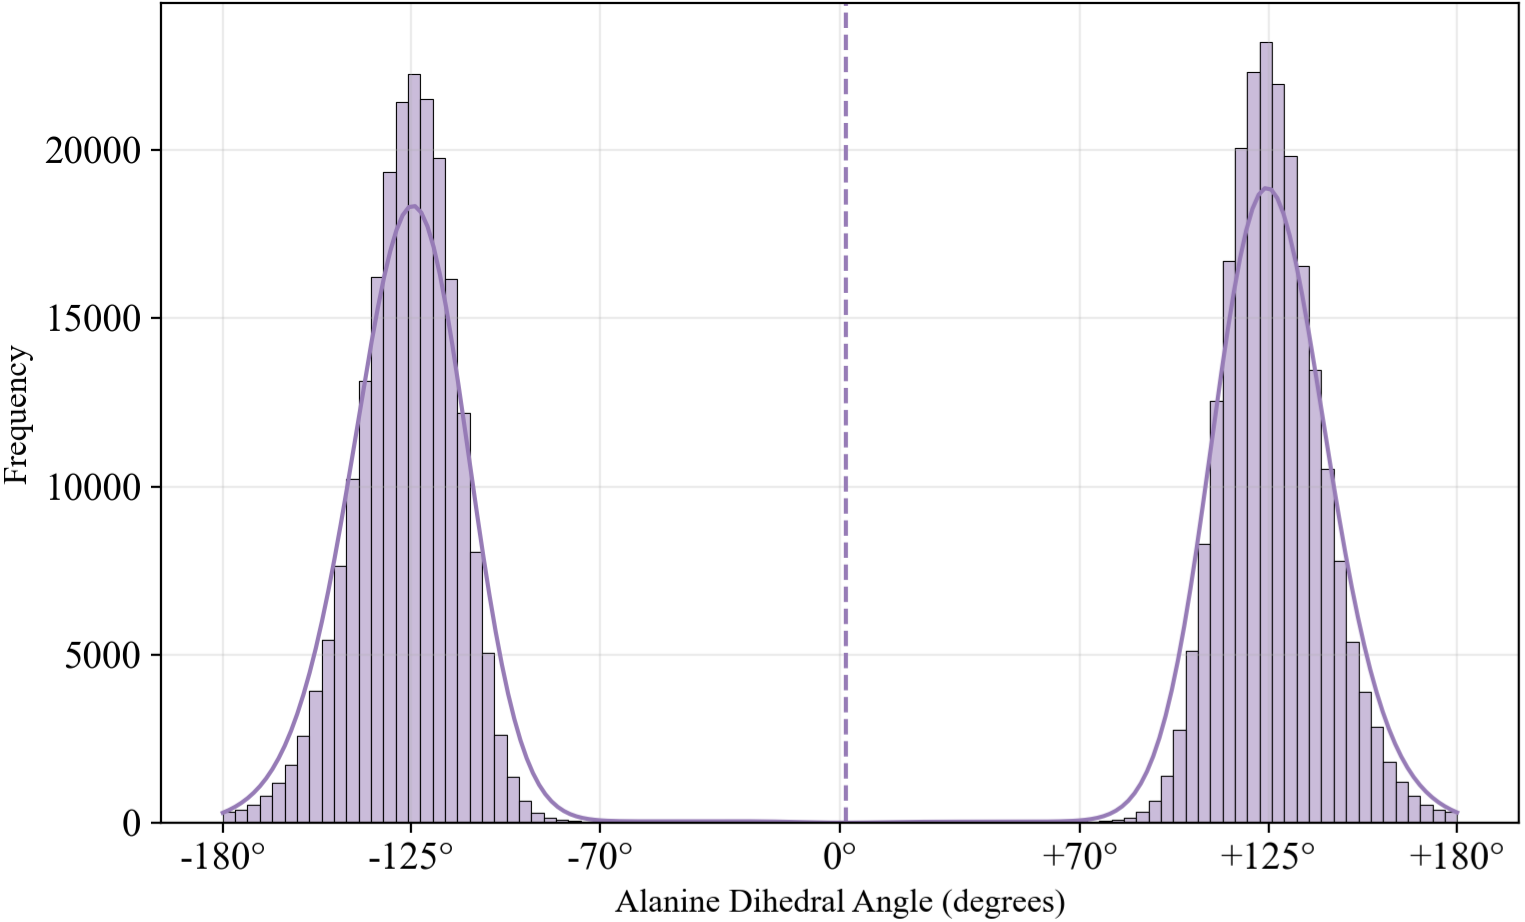
\includegraphics[width=1\linewidth]{Images/alanine_dihedral/alanine_dihedrals_updated.png}
    \caption[Distribution of synthesized alanine dihedral angles]{Distribution of dihedral angles in alanine molecules synthesized in the early earth simulation run ($N=$ 438,370). Structures obtained from the initial graph search, post-processed with refined graph matching. All molecules fall within the expected range of dihedral angles, centered at $\pm$125$^\circ$.}
    \label{fig:ala_dihedral}
\end{figure}

The distribution in Figure \ref{fig:ala_dihedral} shows a mean value of 1.65\textdegree, demonstrating that D and L-alanine are synthesized in nearly equal proportions. 
Further, the dihedral angles cluster around $\pm$125$^\circ$, consistent with expected alanine geometries.
It is important to note here that the difference in plotted values  here ($N=$ 438,370) and the updated GraphMatcher output ($N=$ 445,342) is due to filtering out structures identified along the periodic boundary. 
The RMSD (Equation \ref{eq:rmsd}) of the extracted alanines was compared by computing the average coordinates $\mathbf{r}^{\text{ref}}$ over all structures in the set and comparing each structure to this average reference.
The distribution of RMSD values per-molecule are provided in Figure \ref{fig:ala_rmsd}. 

\begin{equation}
\label{eq:rmsd}
    \text{RMSD} = \sqrt{\frac{1}{N} \sum_{i=1}^{N} \left| \mathbf{r}_i - \mathbf{r}_i^{\text{ref}} \right|^2 }
\end{equation}


\begin{figure}[!ht]
    \centering
    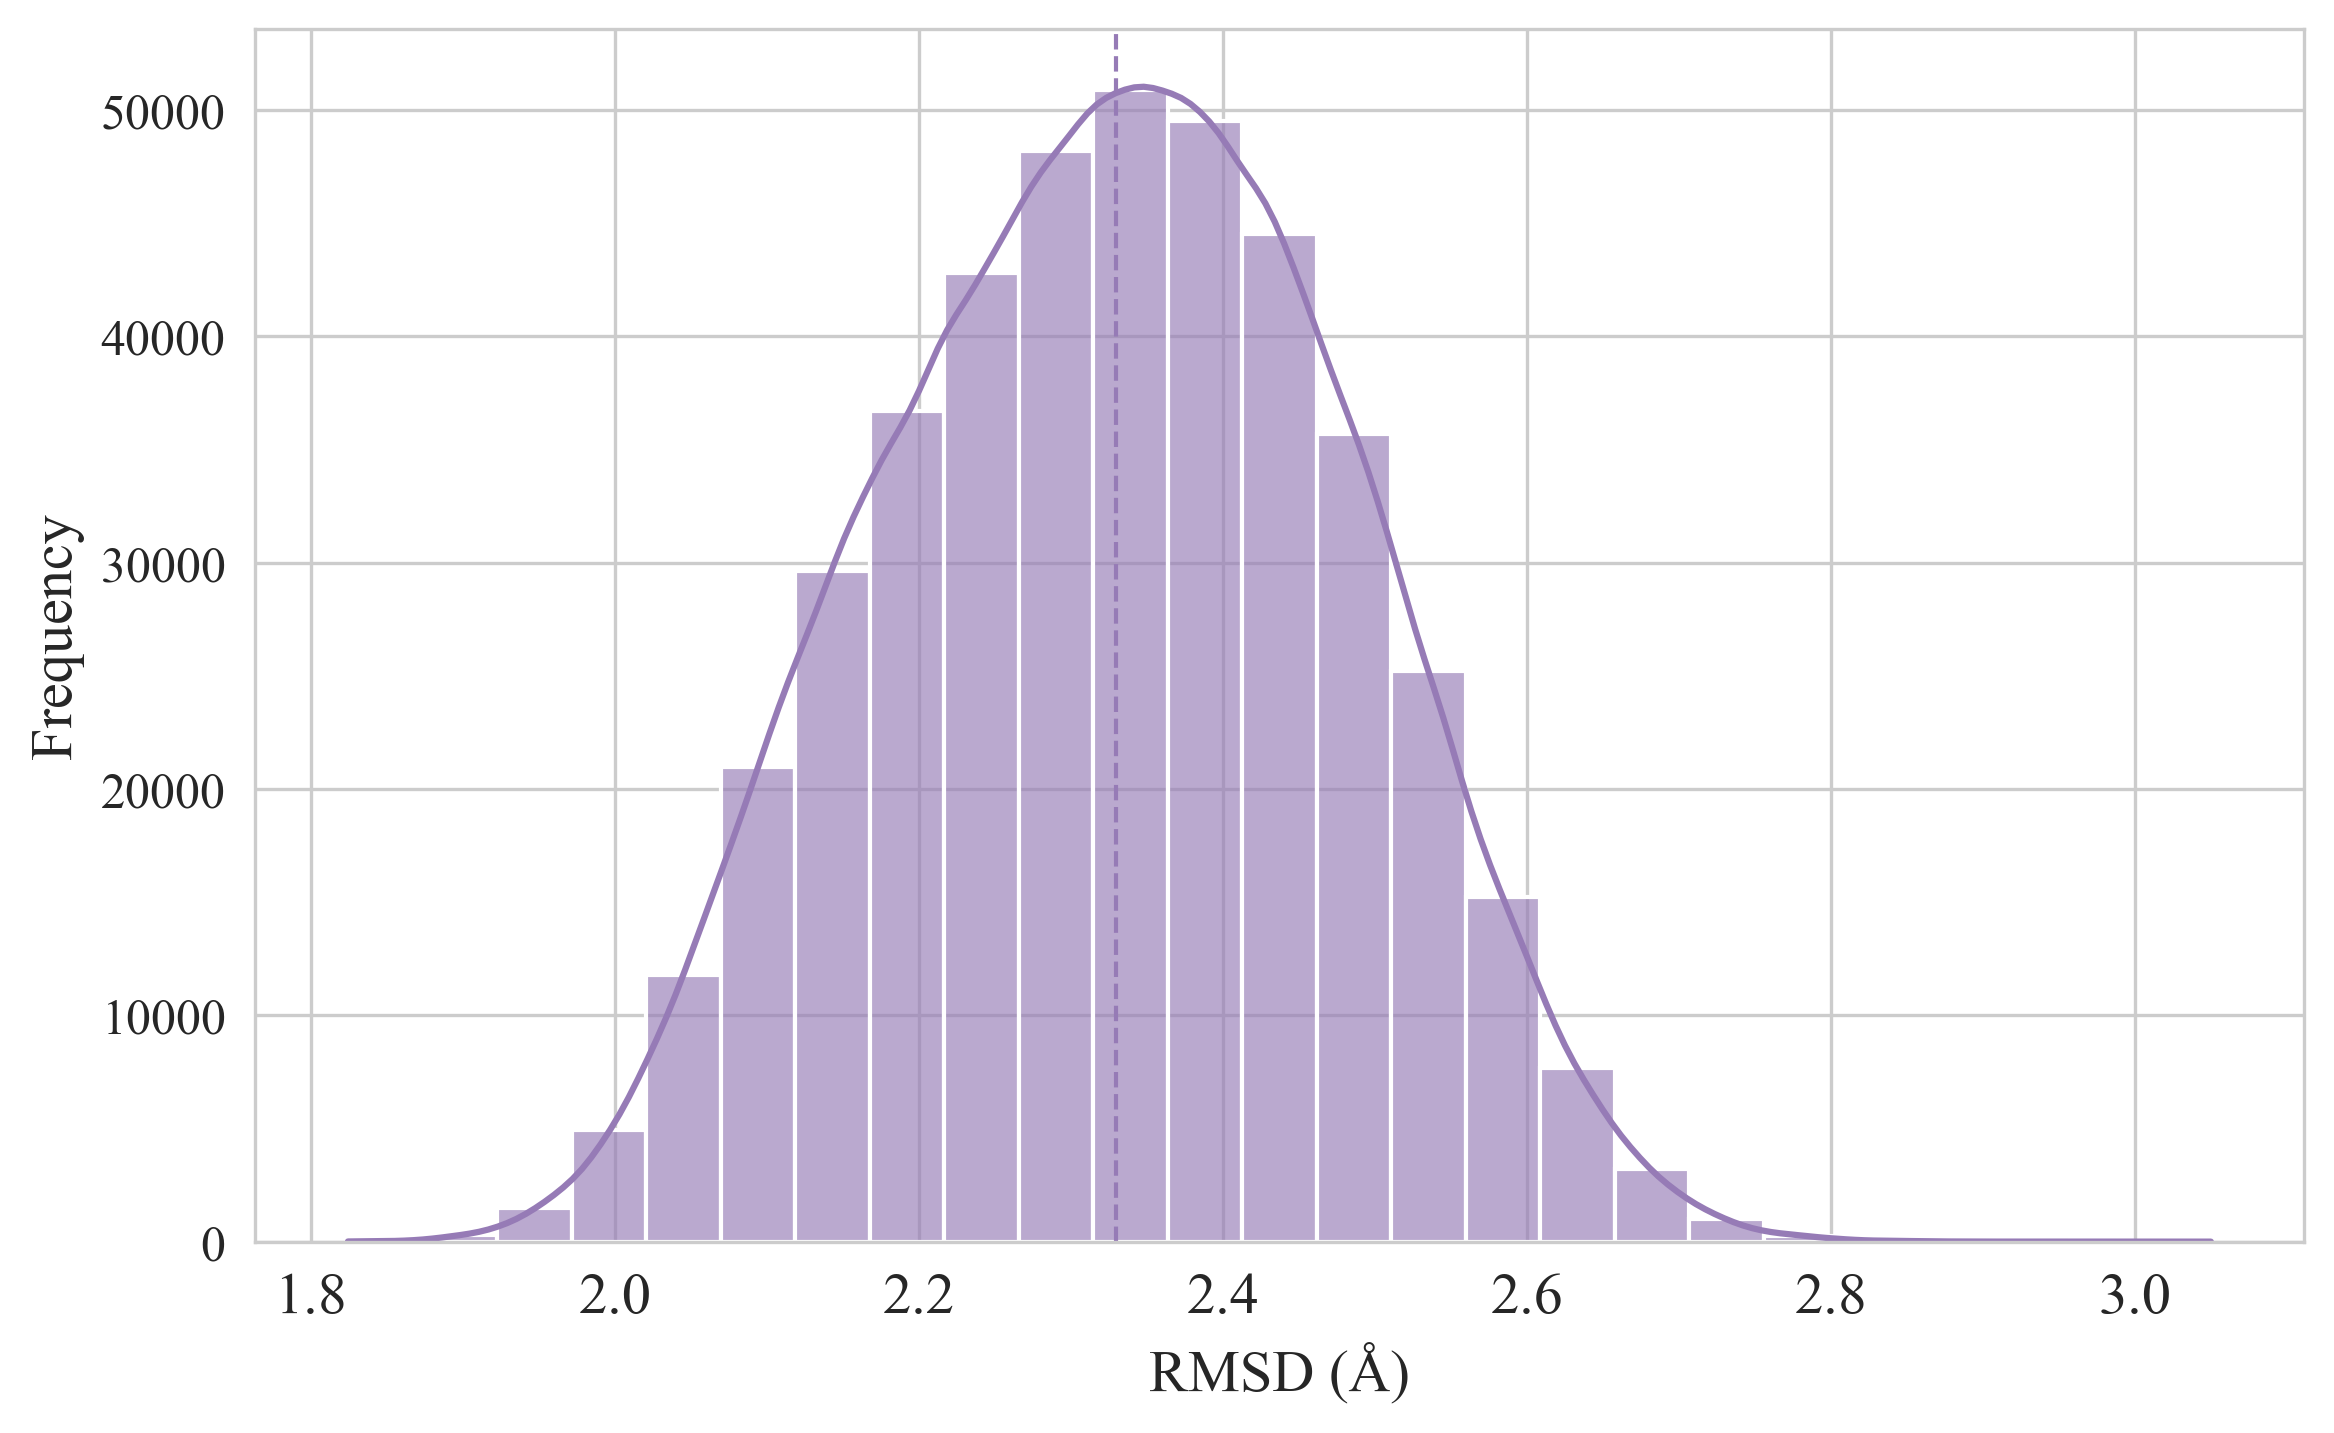
\includegraphics[width=1\linewidth]{Images/alanine_dihedral/rmsd_distribution.png}
    \caption[RMSD of synthesized alanine structures]{Distribution of RMSD values comparing each synthesized alanine to the \textit{average} alanine structure. ($N=$ 438,370, Mean RMSD = 2.33 $\angstrom$)}
    \label{fig:ala_rmsd}
\end{figure}

This analysis confirms that the molecular structures identified through the refined graph search not only match the expected connectivity patterns but also exhibit realistic conformational behavior, further validating the accuracy of the updated graph-matching approach and the chemical validity of products synthesized throughout this large-scale reactive simulation.

\subsection{Preprocessing and Efficiency}
\label{subsec:molfind_parallelization}

The RAPIDS ecosystem \cite{rapids} streamlines the fragmentation and analysis of large-scale reactive MD trajectories like the Hero Run simulation.
Using GPU-accelerated libraries, specifically \verb|cuGraph| and \verb|cuDF|, we can minimize CPU bottlenecks and perform large-scale graph analysis in parallel on GPUs. 
The first part of the \verb|molfind| workflow consists of constructing a singular graph object containing every atom in a frame, splitting that graph into molecular fragments based on distances between atoms, and analyzing connectivity to identify molecules that match a reference structure. 
The \verb|find_fragments| portion of the \verb|molfind| protocol is the rate-limiting step, taking $\sim$9.3 seconds per frame. 
These operations are executed using \verb|cuGraph|, which provides highly optimized, massively parallel algorithms for graph operations.
Instead of iterating through millions of atomic interactions on the CPU, the connected component search in \verb|cuGraph| rapidly groups atoms into discrete molecular fragments, enabling rapid classification of structures.
Unfortunately, \verb|cuGraph| lacks unique graph operations (\textit{i.e.}, graph comparisons), meaning data must be transferred to the CPU in order to compare the graph from a molecular fragment to a reference structure with \verb|NetworkX| \cite{networkx}.

The initial version of \verb|molfind| migrates all fragments with formulas that match an entry of the PubChem database to the CPU and iterates over each group of fragments (with the same chemical formula) to compare each structure within that group to the reference graph.
This works well, but Appendix Table \ref{tbl:formula_vs_mol} shows that with the simplest structure, glycine, only $\sim$26.9\% of structures with formula matches are structurally the same as the reference.
For an average structure in the PubChem, \verb|molfind| has only a $\sim$12.7\% chance of correctly identifying a fragment based on the formula alone.

With the help of Dr. Melisa Alkan from NVIDIA, additional string preprocessing on the GPU was implemented to filter the total number of fragments we compare to reference structures, before any data is migrated to the CPU.
These preprocessing steps included loading all reference graphs into memory, counting the edges (number of bonds) in each reference structure, and discarding the fragment graphs which have a formula that matches an entry of the PubChem dataset but have a different number of edges than the reference structure.
These are recent developments that have been untested on the entire trajectory, but small-scale trials show that these changes decrease the time to analyze each frame, along with a lower fail rate for matching molecules based on the fragment formula.


\section{Restarts: Quench Analysis}
\label{sec:restarts_quench_analysis}

Chemical behavior is very volatile at 2500 K, and synthesized molecules tend to not linger for very long.
To test the stability of synthesized molecules, we selected 415 frames to quench from 2500 K to 300 K as rapidly as possible.
The frames selected were localized to the segments of the simulation held at 2500 K, between 0.2 and 4.2 ns.
Of these, 15 frames were hand-picked: one frame with the highest number of named molecules, one with the most molecular fragments, one containing the largest synthesized molecule throughout the simulation, and 12 frames with the highest number of detected alanine molecules.
The other 400 frames were selected using a random number generator to select 10 frames per 0.1 ns split of the trajectory.

To quench each of these frames, the atomic velocities were initialized at 0 K and temperature was set to 300 K, allowing the Langevin thermostat to slow atomic motions as quickly as possible.
The first quench ran for 5000 steps (0.25 fs timestep) taking 56 minutes on 32 GPUs; timestep versus temperature is plotted every 50 steps in Figure \ref{fig:quench_steps} to demonstrate this equilibration around step 1000.
The temperature settled near 300 K by 1000 steps, and comparing the first quenched system at 1000 and 5000 frames shows minimal differences in molecular stability.
This was the timescale used for quenching the remaining 414 selected frames.

\begin{figure}[!ht]
    \centering
    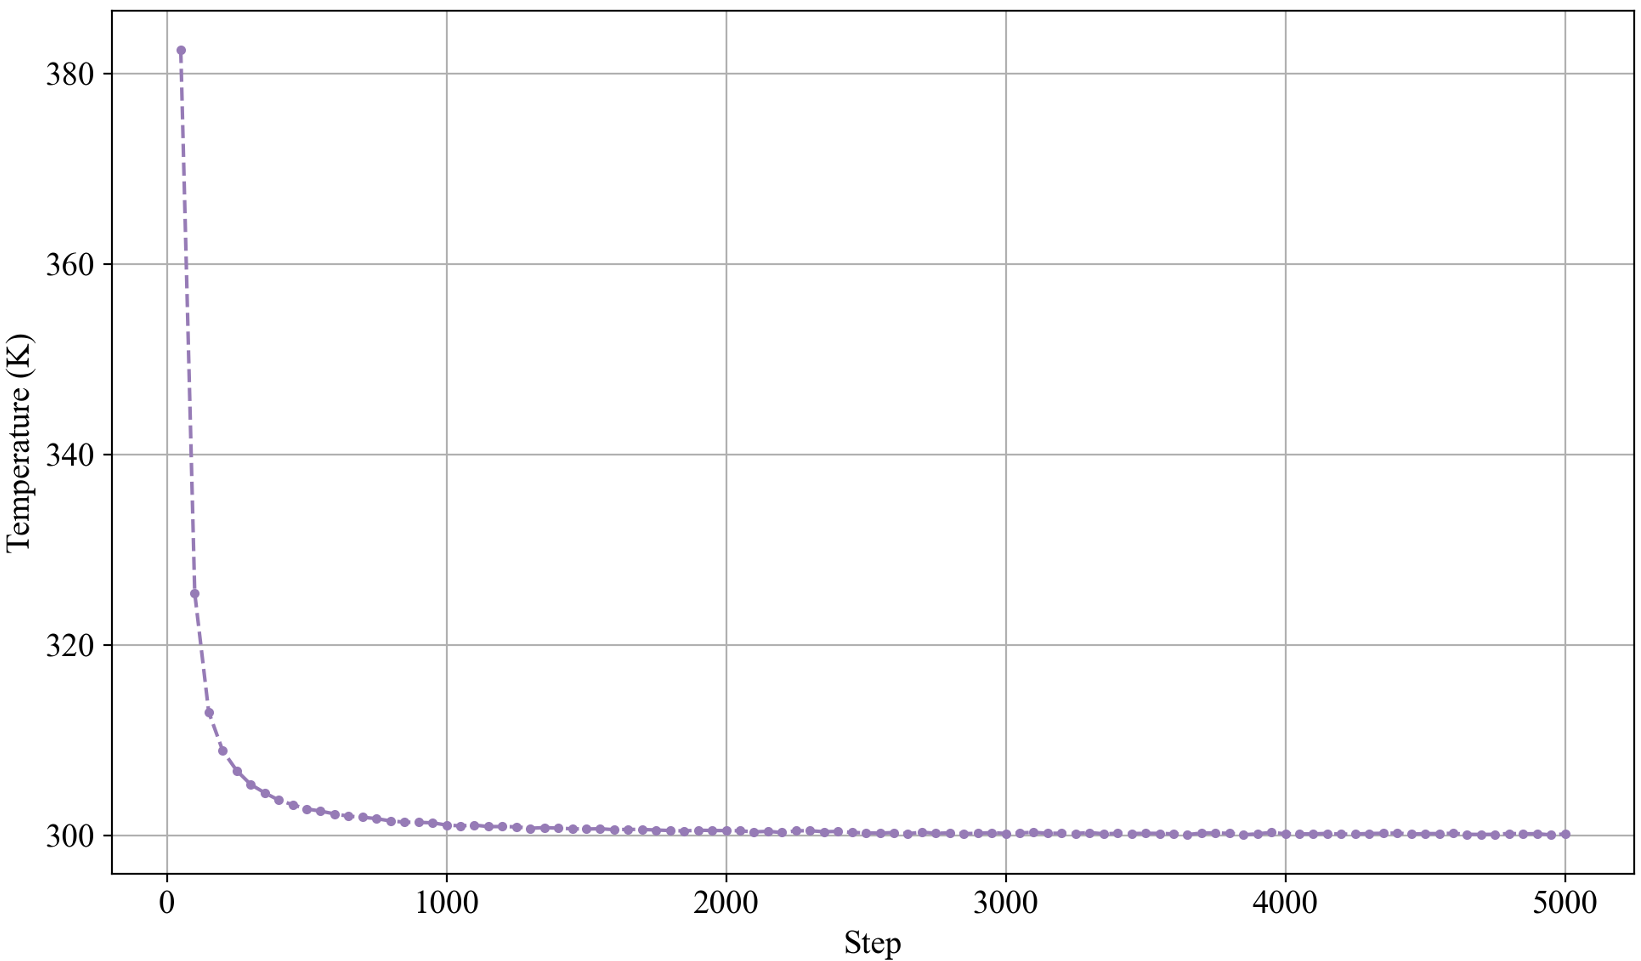
\includegraphics[width=1\linewidth]{Images/early_earth/steps_vs_temp_quench.png}
    \caption[MD steps required to quench system]{Timestep versus temperature for quenching Hero Run frame from 2500 K to 300 K. The temperature is first measured by LAMMPS at 382.5 K due to initializing the velocities at 0 K.}
    \label{fig:quench_steps}
\end{figure}

Each of these quench runs took an average of 15 minutes and 51 seconds, requiring 32 GPUs to avoid hitting memory caps.
The system could initialize on only 24 GPUs, however after a few frames every run encountered memory issues while running dynamics.
The histograms in Figure \ref{fig:ee_quench_hist} compare the distribution of named molecules before and after quenching, highlighting a significant increase in named molecules found after quenching.

\begin{figure}[!h]
    \centering
    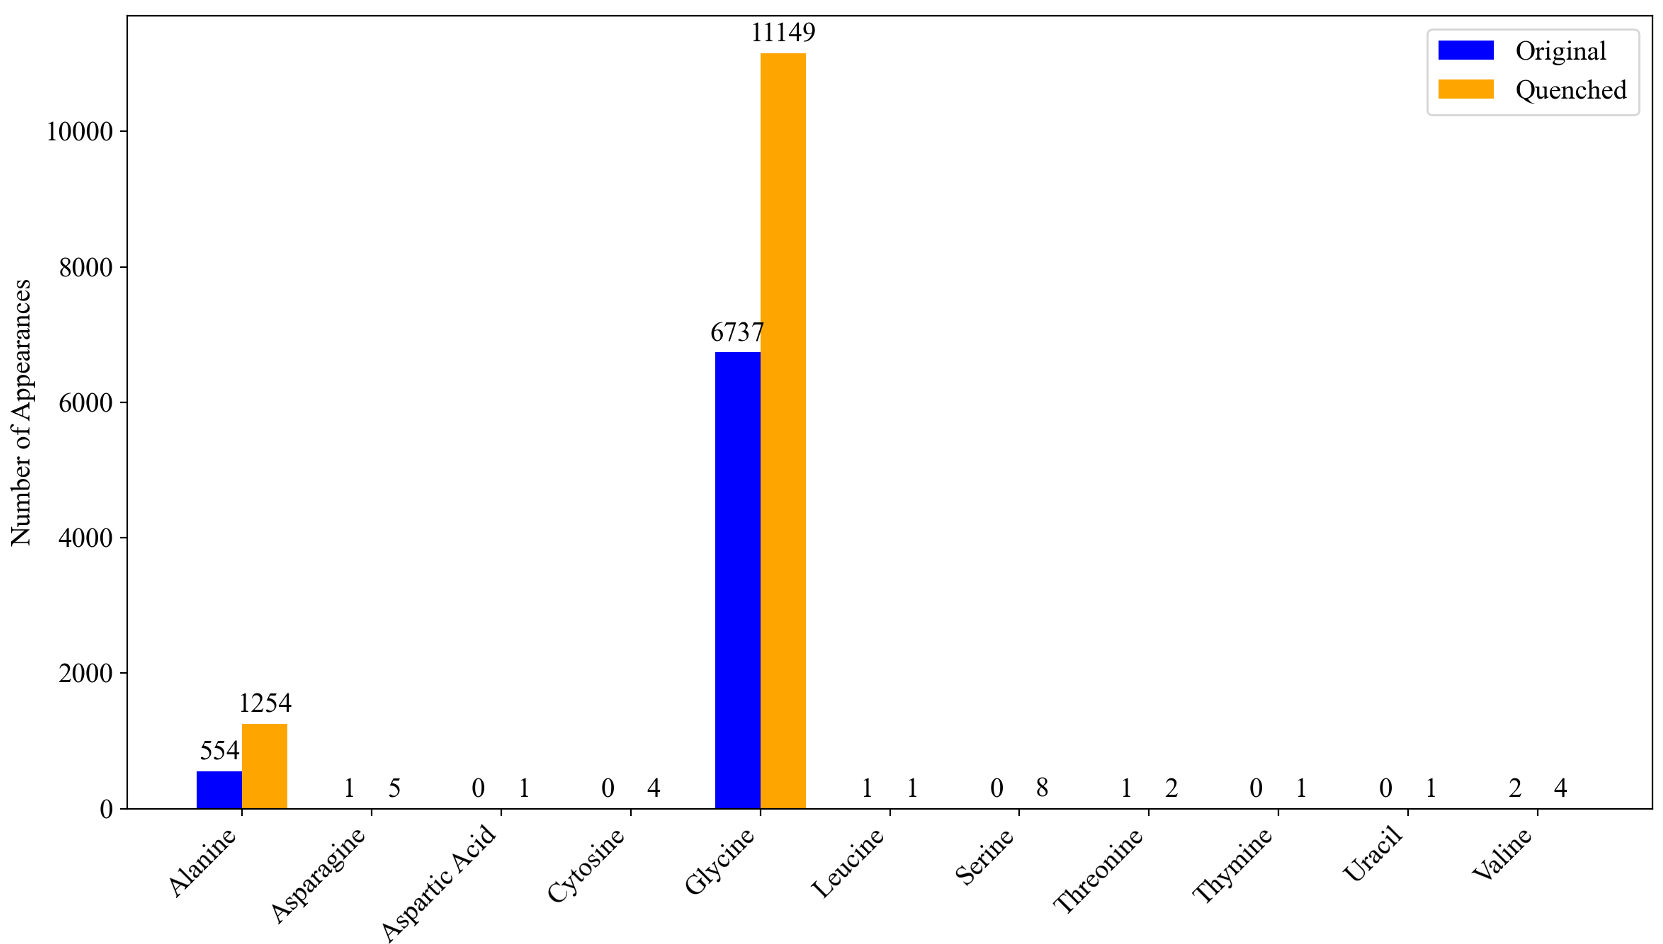
\includegraphics[width=1\linewidth]{Images/early_earth/mol_before-after_quench.png}
    \caption[Histogram: molecules found before and after quenching system]{Histogram of named molecules found before and after quenching 415 selected frames from the 22.8M atom system from 2500 K to 300 K.}
    \label{fig:ee_quench_hist}
\end{figure}

We note the appearance of several molecules that were not detected at 2500 K.
None of the quenched frames showed a disappearance of a named molecule after cooling, which speaks to the stability of the synthesized molecules.
This increased detection is further illustrated in Figure \ref{fig:ee_quench_lineplot}, which tracks the total count of named molecules per-frame before and after the quench. 
Prior to quenching, there was an average of 18 named molecules per frame.
While the total number of individual fragments decreased after cooling, the presence of larger, more chemically diverse molecules increased, indicating that higher-order molecular assembly is favored at lower temperatures.

\begin{figure}[!h]
    \centering
    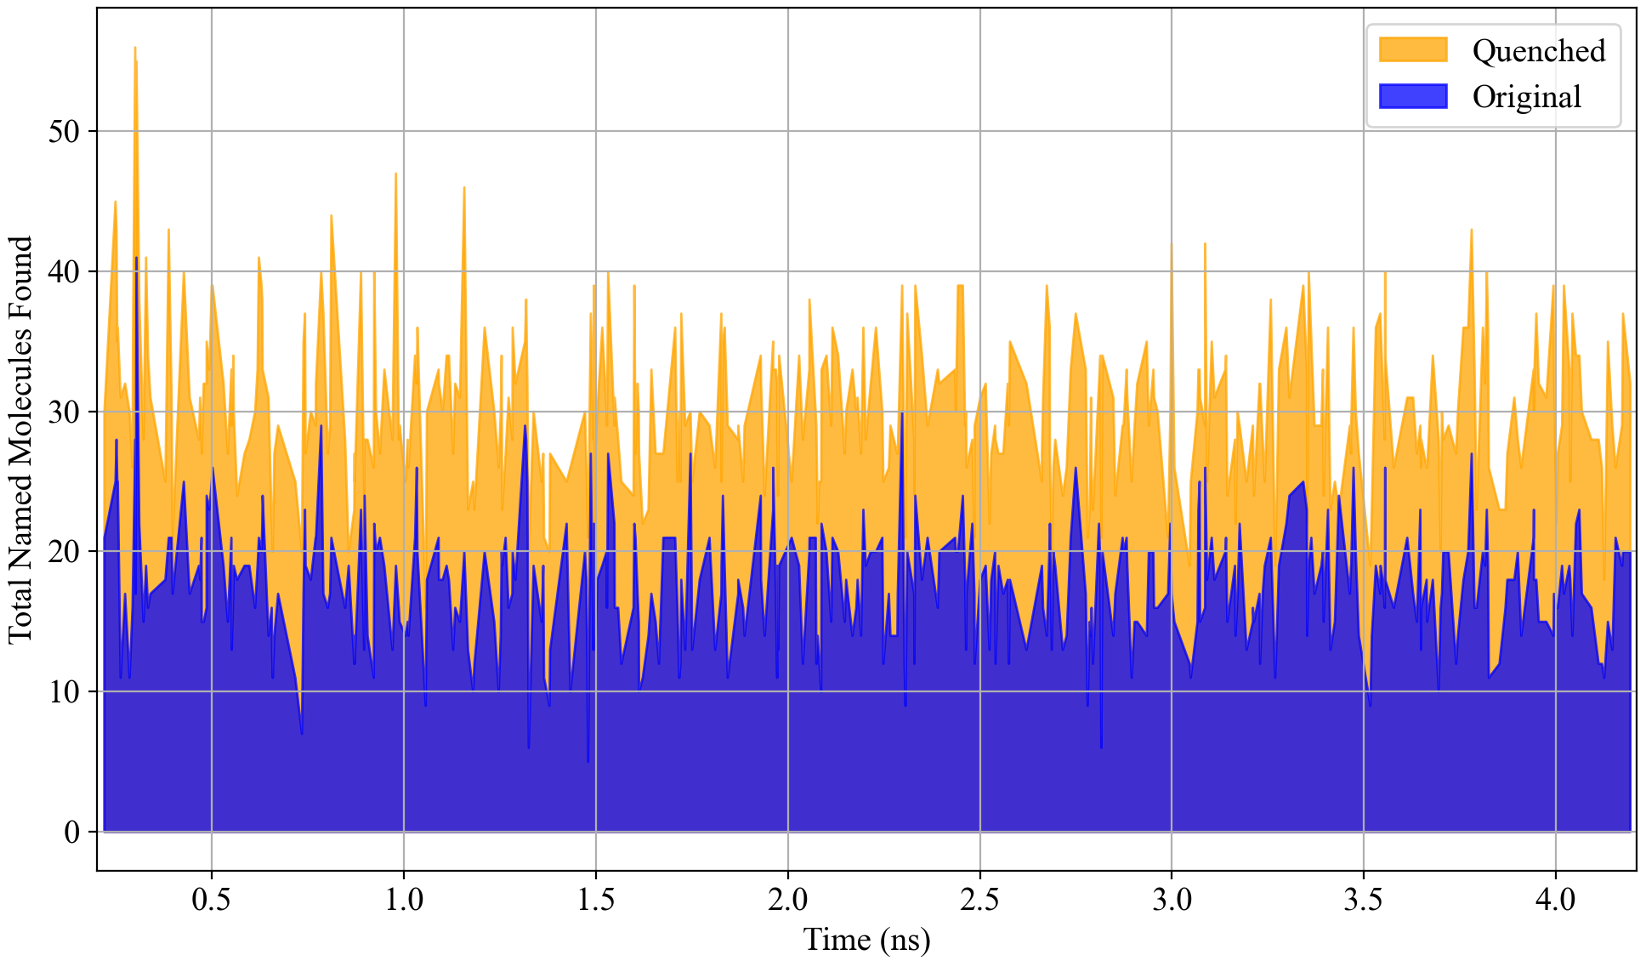
\includegraphics[width=0.885\linewidth]{Images/early_earth/named_mols_before-after_quench.png}
    \caption[Line plot: total named molecules found before and after quenching system]{Total per-frame count of named molecules found before and after quenching 415 selected frames from the 22.8M atom system from 2500 K to 300 K.}
    \label{fig:ee_quench_lineplot}
\end{figure}

Following the temperature drop, the system shifts toward larger and more stable molecular species, increasing to an average of 30 named molecules in each frame as shown in Figure \ref{fig:ee_quench_violinplot}.

\begin{figure}[!ht]
    \centering
    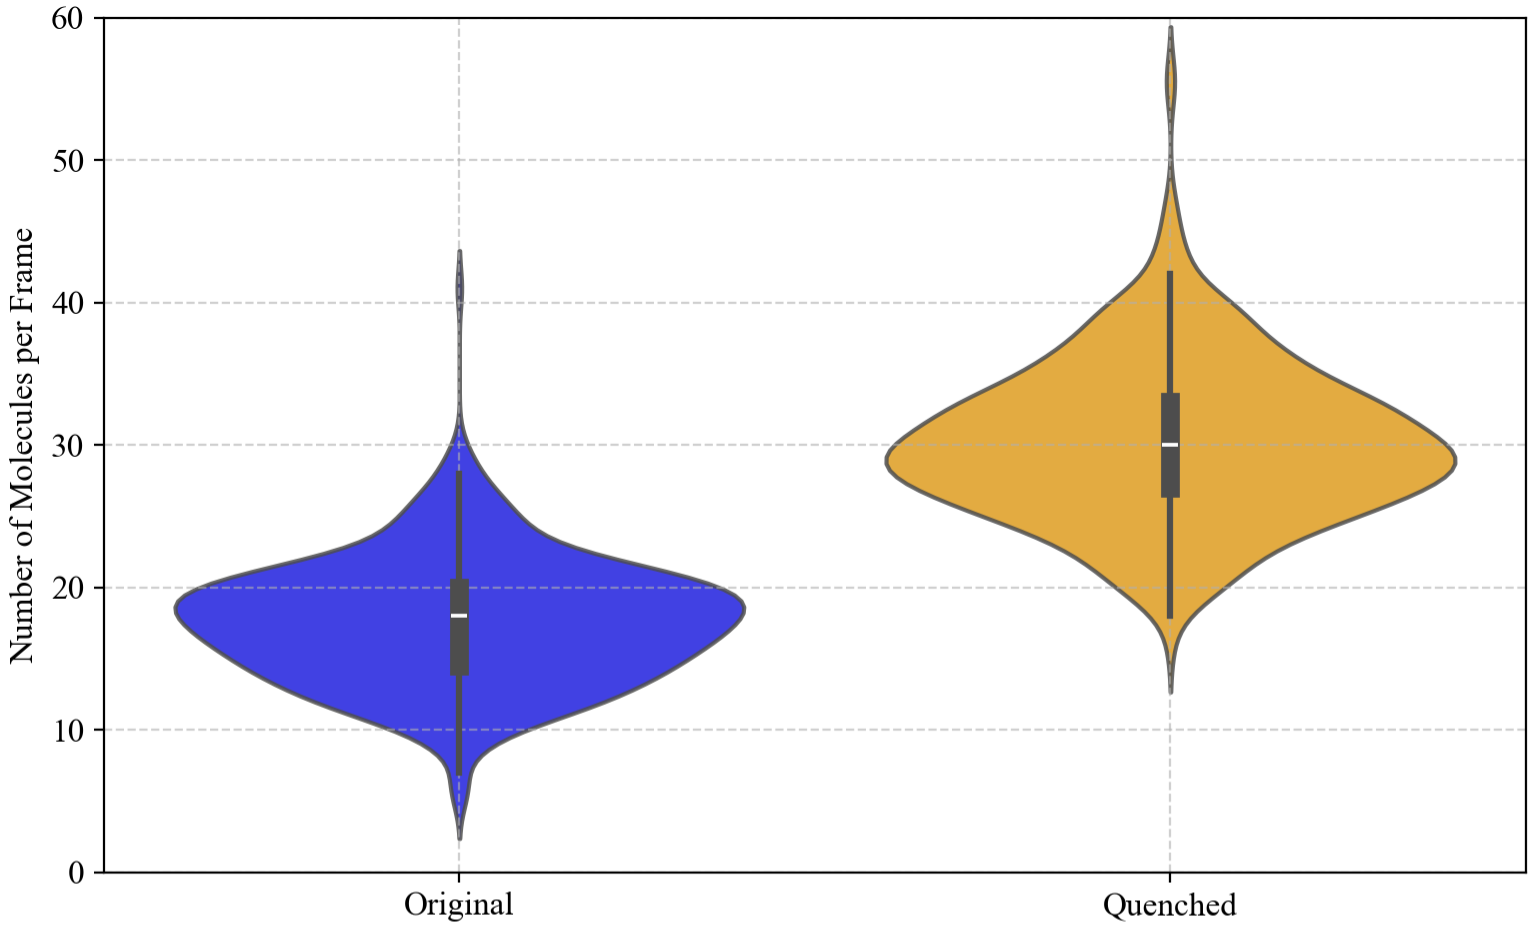
\includegraphics[width=0.885\linewidth]{Images/early_earth/updated_violins.png}
    \caption[Violin plot: total named molecules found before and after quenching system]{Distribution of per-frame counts of named molecules found before and after quenching 415 selected frames from the 22.8M atom system from 2500 K to 300 K.}
    \label{fig:ee_quench_violinplot}
\end{figure}

To form larger fragments, the low molecular weight formulas quickly combine into larger fragments, which can be seen by visualizing the total number of unique chemical formulas in each frame.
This trend is shown in Figure \ref{fig:quench_unique_formulas}.

\begin{figure}[!ht]
    \centering
    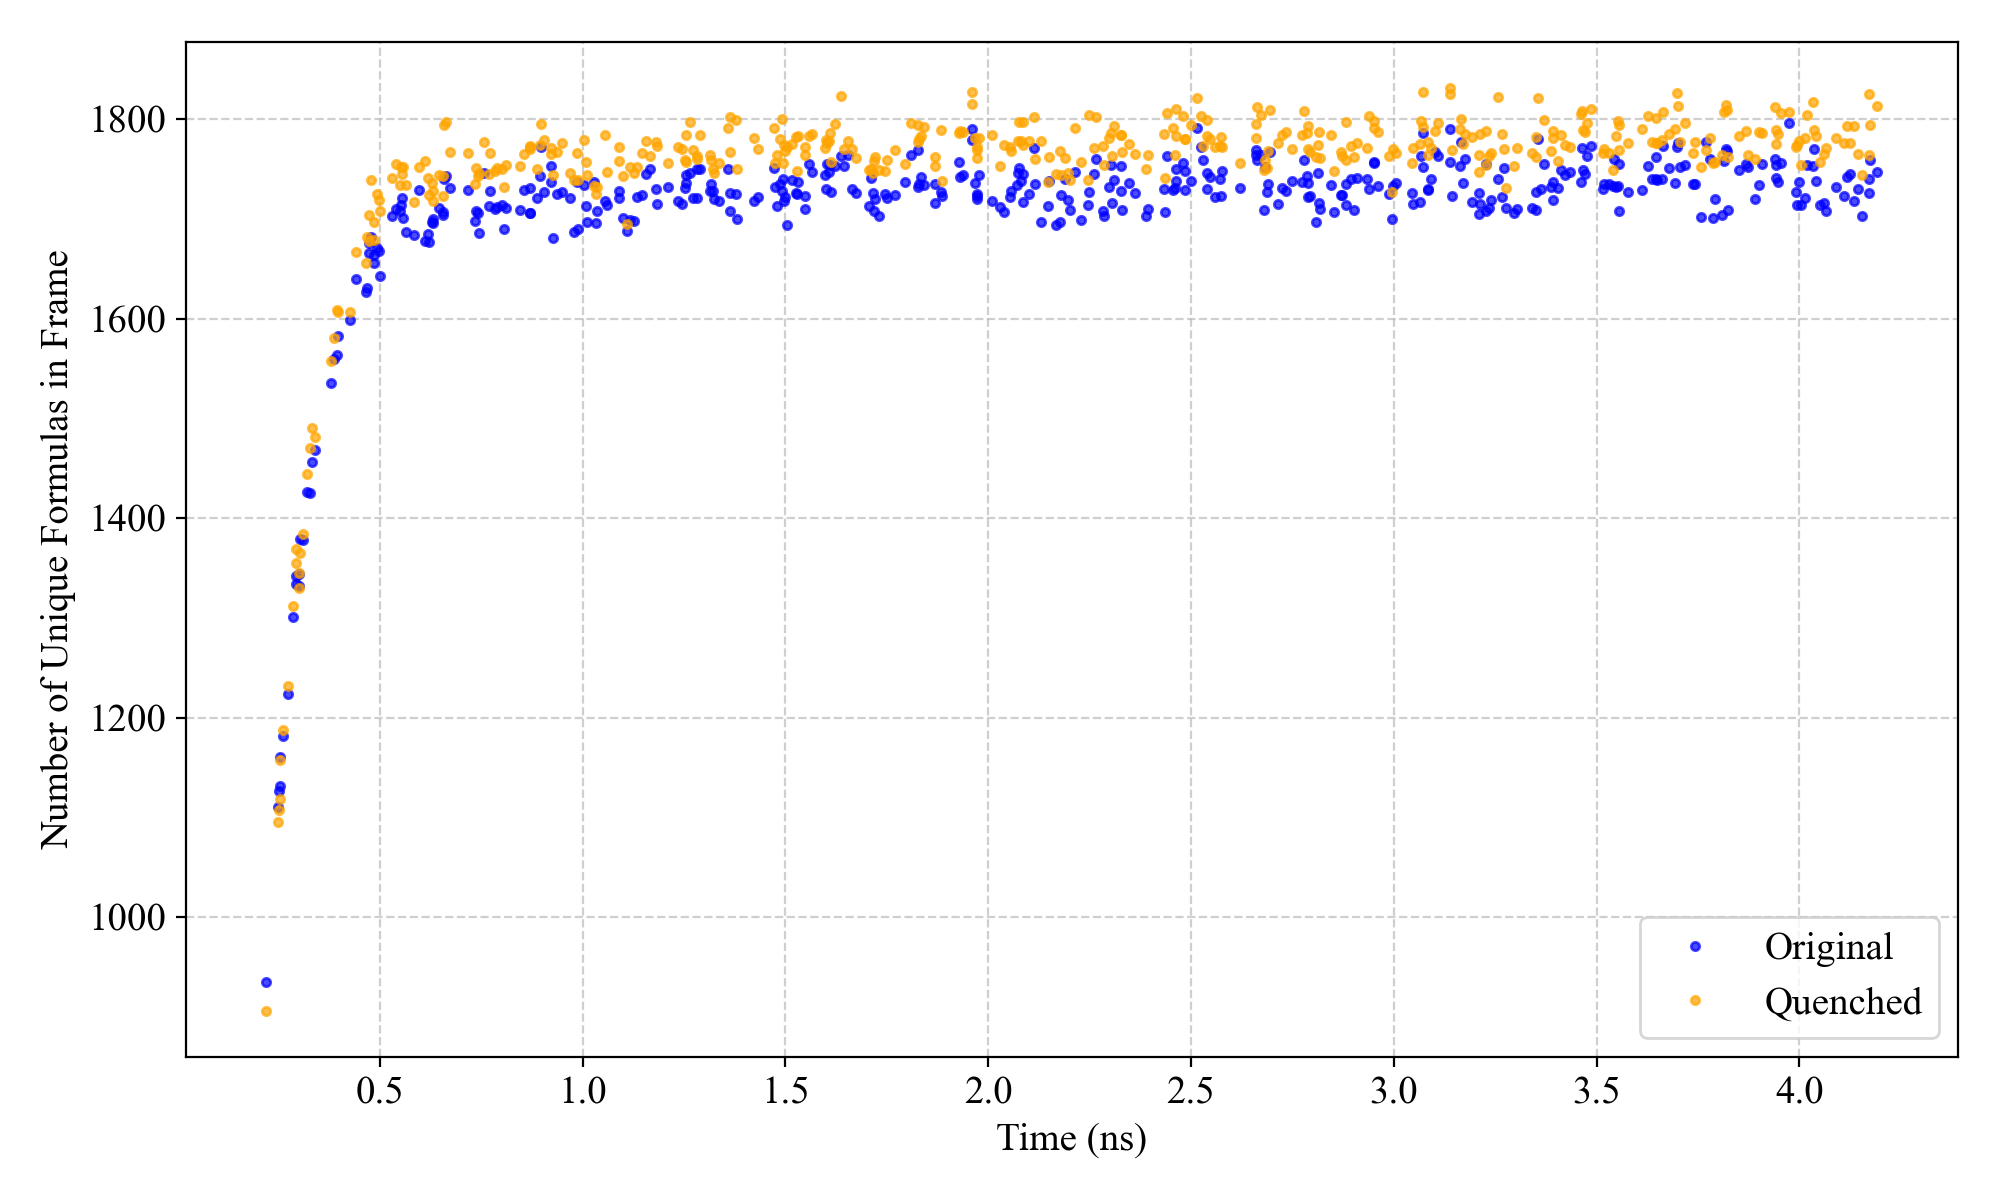
\includegraphics[width=1\linewidth]{Images/early_earth/quench_formula_vs_frame.png}
    \caption[Unique formulas before and after quenching system]{Unique formulas before and after quenching 415 frames of the Hero Run system. The number of chemical formulas present in each frame increases as the system cools, suggesting that small fragments (which are far more abundant) assemble into larger fragments as the temperature drops.}
    \label{fig:quench_unique_formulas}
\end{figure}

Rapidly quenching the system from 2500 K to 300 K shows that high-temperature conditions promote fragmentation and chemical diversity, while cooling allows for stabilization and aggregation into more intricate molecules.
This approach could be applied to sampling complex molecular configurations from simulations of prebiotic chemistry, where transient high-energy environments could generate molecular building blocks that later assemble under cooler conditions into a highly diverse set of stable organic structures.

\section{Exploring New Molecular Configurations}
\label{sec:exploring_new_mol_configs}

As mentioned in Subsection \ref{subsec:drawback_config_sampling}, configurational diversity is difficult to implement in the active learning via query by committee used in generating ANI datasets, and as a result new molecular configurations have been sampled from enumeration datasets and other curated chemical datasets.
The ANI-1xnr \cite{ani-1xnr} approach to generating training set data via nanoreactors serve as an inspiration for sampling new configurations from a massive batch of reactive molecular dynamics data.
Identifying all of the molecular species synthesized throughout the Hero Run simulation is a step toward using this data to refine the behavior of the NNP model.

Unique graph operations are unavailable on GPUs, and migrating every molecular fragment graph in each frame to the CPU in order to determine the total number of unique fragments in a frame is computationally prohibitive.
Instead, in order to capture structural details beyond composition for molecules outside of the PubChem dataset, we implemented a “signature” string that encodes the internal connectivity of each molecule. 
Each bond is represented in a standardized format (\textit{e.g.}, sorted alphabetically as ``C-H'', ``H-O'', etc.) and aggregated to form a reproducible fingerprint. 
This combination of stoichiometric and connectivity descriptors ensures that fragments with identical compositions but different bond arrangements can be distinguished. 
It is important to note that this approach is not as comprehensive as direct graph comparisons, but it captures the same level of detail as the original \verb|molfind| by identifying which bonds exist within a graph. 
We still aggregate molecules with the same formula which have differences in configuration, but this is the most refined approach that could be implemented entirely on GPU.

This approach increases the time to analyze each frame from 9.93 to 10.24 seconds, but gives much more refined information about each fragment within the frame.
The disk space occupied by the output \verb|df_formula| parquet also increases by a factor of 15.3x by storing this extra data, from $\sim$2.5 GB to nearly 40 GB, in turn occupying even more memory when unpacked into a data frame.
The complication working with a data frame of this magnitude (557 million rows) is that \verb|Pandas| \cite{pandas}, which is typically a go-to library for Python-based data analysis, creates copies of the data frame object in memory in order to perform operations.
Using a dynamic library like \verb|Dask| \cite{dask} circumvents this limitation by distributing the analysis across multiple processing units and scheduling tasks for data manipulation. 
An example of the signatures assigned to each structure are provided in Table \ref{tbl:unique_signatures_start}.

\begin{table}[h!]
\centering
\caption[Example of molecular fingerprint]{Example of molecular fingerprint strings assigned to each molecule. Molecules shown here are the five starting materials, along with the total appearances of each molecule throughout the 4.4 ns simulation and the average number times each molecule appears per frame.
}\label{tbl:unique_signatures_start}
\begin{tabularx}{0.85\textwidth}{llrr}  
\toprule
Molecule & Signature & Total appearances & Per-frame \\
\midrule
\ce{H2O} & \verb|HHO_H-O_H-O| & 599,974,869,205 & 1,704,474 \\
\ce{CH4} & \verb|CHHHH_C-H_C-H_C-H_C-H| & 326,456,352,440 & 927,432 \\
\ce{NH3} & \verb|HHHN_H-N_H-N_H-N| & 283,123,115,083 & 804,327 \\
\ce{H2} & \verb|HH_H-H| & 242,625,414,453 & 689,276 \\
\ce{CO} & \verb|CO_C-O| & 58,501,381,388 & 166,197 \\
\bottomrule
\end{tabularx}
\end{table}

In total, more than 1.1 million unique molecular signatures were assigned throughout the 4.4 ns simulation. 
By aggregating molecular connectivity data in this way, the evolution of molecular diversity can be tracked.
Figure \ref{fig:unique_signatures} shows the number of new unique signatures versus time, showing how new molecular configurations are more common as soon as the simulation reaches 2500 K but chemical diversity is still being explored when the system begins cooling to 300 K.

\begin{figure}[!ht]
    \centering
    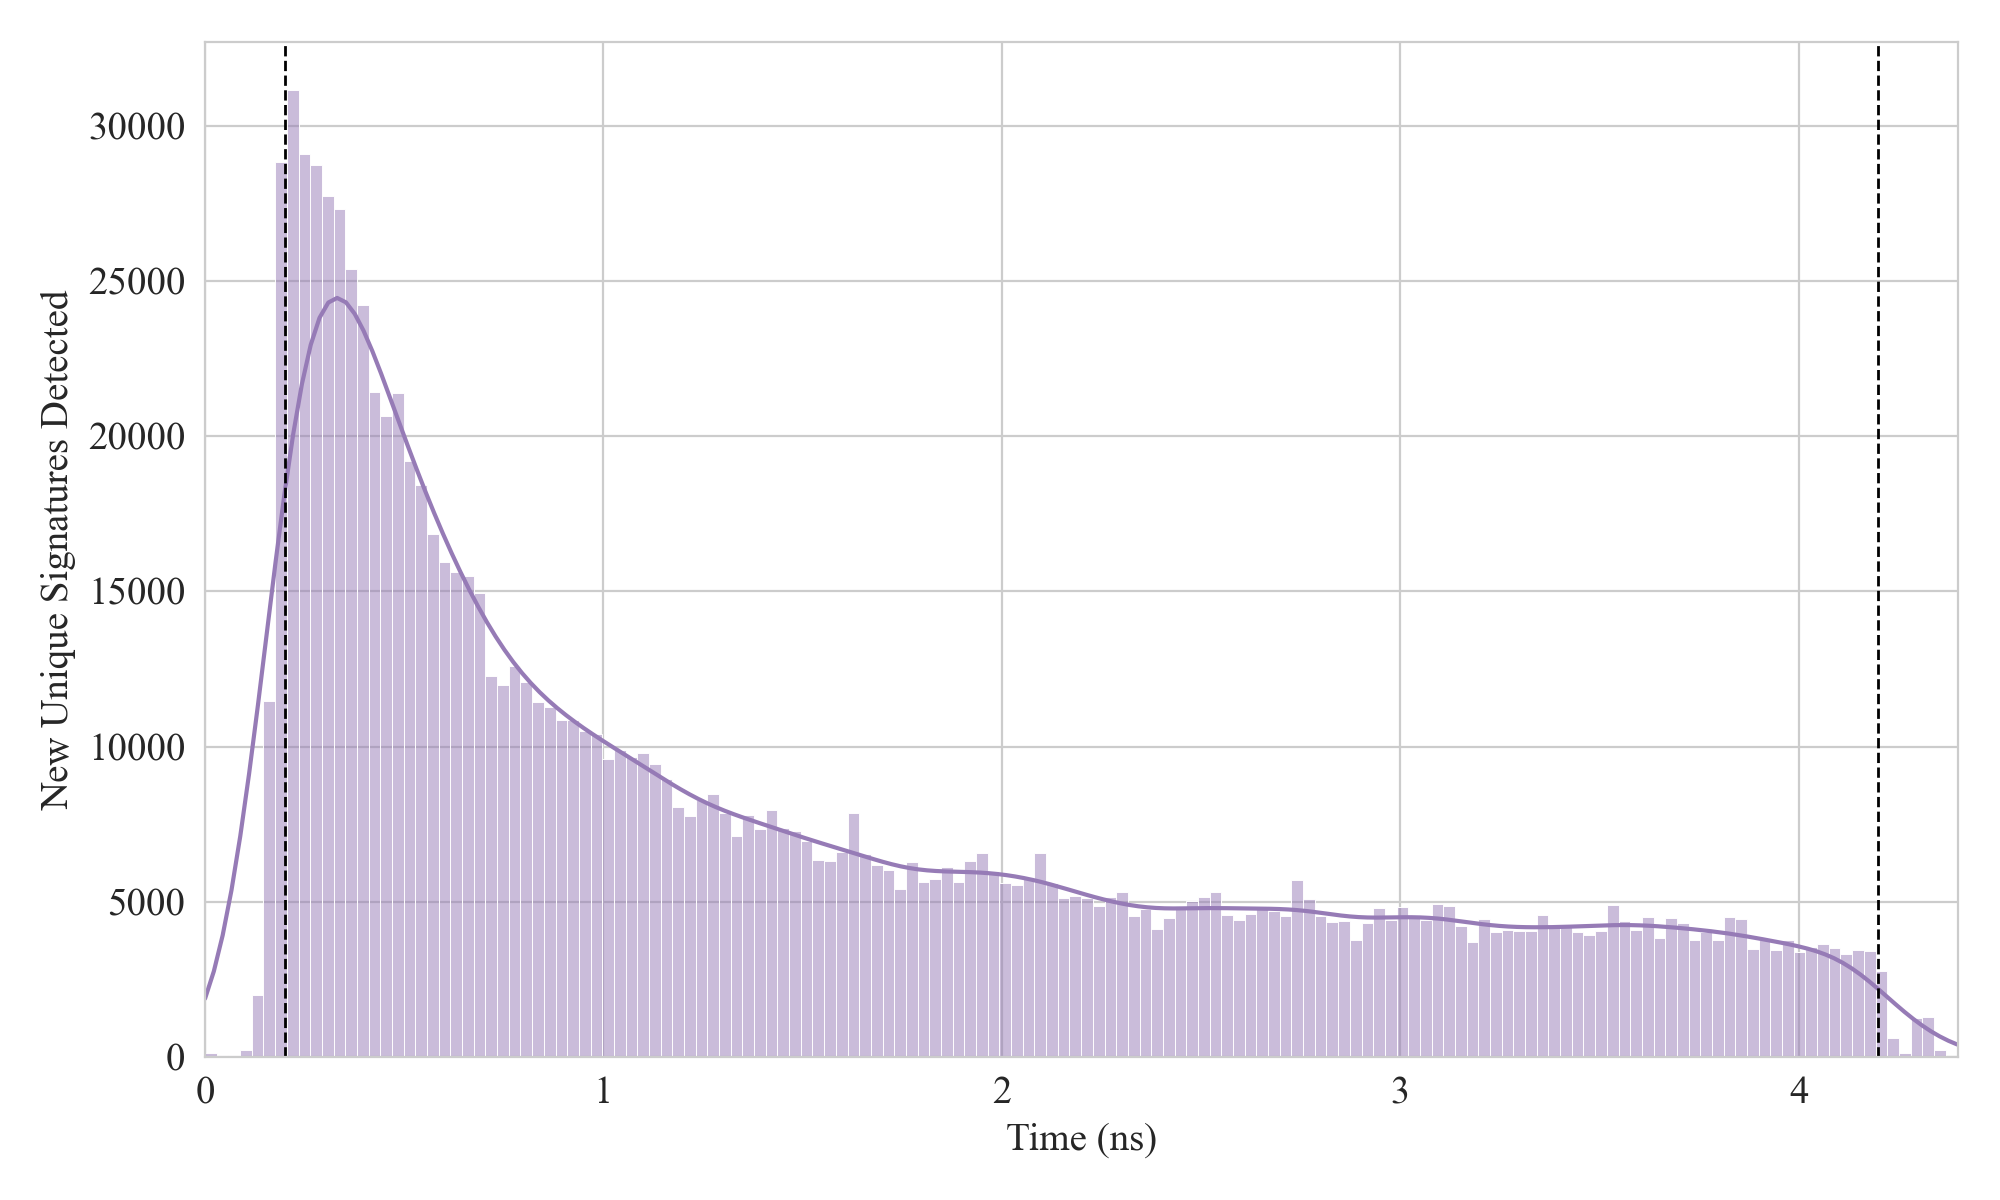
\includegraphics[width=1\linewidth]{Images/early_earth/unique_signature_vs_time.png}
    \caption[Molecular fingerprints throughout the Hero Run simulation]{New molecular fingerprints, counting the first appearance of each unique signature, versus time ($N=$ 1,119,793). The dotted black lines indicate when the temperature reaches 2500 K (left) and starts cooling back to 300 K (right).}
    \label{fig:unique_signatures}
\end{figure}

Further, by using this data, it is possible to determine the point at which any specific molecule appears for the first time throughout the simulation, or track how many times a molecule of interest forms and how for long it persists. 
This is demonstrated in Table \ref{tbl:signatures_appeared_once}, which shows molecular signatures that appear only once throughout the entire simulation. 
Some of these unique signatures appear shortly after the system begins heating toward 2500 K at 0.1 ns, while other unique signatures are still being detected at 300 K just before the simulation ends.

\begin{table}[h!]
\centering
\caption[Unique molecular fingerprints]{Abbreviated list of molecular fingerprint strings that appeared only once throughout the simulation. In total, 373,537 of the 1,119,793 molecular fingerprints appeared only once.
}\label{tbl:signatures_appeared_once}
\begin{tabularx}{0.85\textwidth}{lr}  
\toprule
Signature & First appearance \\
\midrule
\verb|CCCHHHHHNNOOOO_C-C_C-C_C-N_C-N_C-O_C-O_C-O_H-N...| & 0.114312 ns \\
\verb|CCCHHNNOOOO_C-C_C-C_C-N_C-N_C-O_C-O_C-O_H-N_H-...| & 0.120650 ns \\
\verb|CCCCCHHHHHNOOOOO_C-C_C-C_C-C_C-C_C-H_C-N_C-O_C...| & 0.129687 ns \\
\verb|CCCCCHHHHNOOOOOOO_C-C_C-C_C-C_C-C_C-N_C-O_C-O_...| & 0.131225 ns \\
\verb|CCCCHHHNOOOOOO_C-C_C-C_C-C_C-N_C-O_C-O_C-O_C-O...| & 0.132513 ns \\
... & ... \\
\verb|CCCCCCCCCCCCCCCHHHHHHHHHHHHHHHHHHHHNNNOOO_C-C_...| & 4.392288 ns \\
\verb|CCCCCCCCCCCCCCCHHHHHHHHHHHHHHHHHHHHHNNNNOO_C-C...| & 4.392962 ns \\
\verb|CCCCCCCHHHHHHHHHHNNOO_C-C_C-C_C-C_C-C_C-C_C-C_...| & 4.396262 ns \\
\verb|CCCCCCCCCCCCCHHHHHHHHHHHHHHHHNO_C-C_C-C_C-C_C-...| & 4.396625 ns \\
\verb|CCCCCCCCCCCHHHHHHHHHHHHHHHHHNNOOO_C-C_C-C_C-C_...| & 4.398237 ns \\
Total: 373,537 signatures & -- \\
\bottomrule
\end{tabularx}
\end{table}

This approach to assigning signatures to each molecule aids in analyzing and understanding the chemical diversity sampled throughout the Hero Run simulation.
The next steps to extract more useful data was to expand the list of molecules of interest in the PubChem dataset.

\section{Expanding the Search}
\label{sec:expanding_the_search}

In the initial search, the PubChem dataset contained 357 molecules.
Of these, 324 molecules were dipeptides, assembled from all possible pairs of proteinogenic amino acids.
As ANI-1xnr is trained only on the H, C, N, O atom types, we exclude cysteine and methionine, which contain sulfur.
Using the initial PubChem dataset, only 18 of the 357 molecules are found throughout the simulation.
Further, of the possible 324 combinations of dipeptides, only glycylglycine is detected.
This set of molecules is too restrictive to detect all biologically relevant molecules sampled throughout the simulation. 
To broaden the molecular search beyond simple biological molecules, we looked to publications about prebiotic chemistry and the origin of organic compounds in astrochemical systems.

Recent analysis of samples from the asteroid Bennu (101955) has revealed an abundance of organic matter, including amino acids, carboxylic acids, polycyclic aromatic hydrocarbons, and N-heterocycles, suggesting that the formation of such prebiotic molecules is possible in gas-phase systems \cite{astroid_sample}.
Additionally, it has been demonstrated \cite{prebiotic_compounds_EE_atmosphere} that prebiotic compounds can form protocell-like structures from the aggregation of polymerized HCN molecules under plausible early Earth atmospheric conditions. 
Each of these studies present new targets for detection with \verb|molfind|; we categorize the new PubChem dataset into seven groups, a summary of this dataset is given in Table \ref{tbl:new_pubchem}.

\begin{table}[h!]
\centering
\caption[Updated PubChem database]{Categories and molecule counts in the updated PubChem dataset.}\label{tbl:new_pubchem}
\begin{tabularx}{0.34\textwidth}{lr}  
\toprule
Category & \textit{N}\textsubscript{molecules} \\
\midrule
\verb|amino_acids| & 18 \\
\verb|dipeptides| & 324 \\
\verb|nucleobases| & 5 \\
\verb|fatty_acids| & 5 \\
\verb|simple_sugars| & 4 \\
\verb|asteroid_data| & 41 \\
\verb|hcn_polymers| & 51 \\
Total: 7 categories & 448 \\
\bottomrule
\end{tabularx}
\end{table}

To expand the PubChem dataset, we must carefully choose molecules which are structurally significant and do not appear so often that we are saving millions of atomic positions per frame, which would effectively just be converting the \verb|dcd| trajectory into a less compressed format.
The update to the Pubchem dataset with \verb|asteroid_data| and \verb|hcn_polymers| initially included 457 molecules, but 9 of the species participating in HCN polymerization were very small molecules that significantly increased the time required to analyze a single frame of the trajectory.
These nine species and the time taken to compare each of them against a reference structure are provided in Table \ref{tbl:full_new_pubchem}.
In total, the addition of the species listed added $\sim$224 seconds to the analysis of a single frame, which takes only $\sim$10 seconds with the original PubChem dataset as a list of reference structures. 

\begin{table}[h!]
\centering
\caption[Small molecules excluded from updated PubChem database]{Small molecules excluded from updated PubChem database, along with the formula and structural matches within a single frame and the time taken to identify each molecule.}\label{tbl:full_new_pubchem}
\begin{tabularx}{0.815\textwidth}{llrrr}  
\toprule
Name & Formula & Formula matches & Structure matches & Time (s) \\
\midrule
Formic acid & \ce{CH2O2} & 6,761 & 6,706 & 11.46  \\
Acetic acid & \ce{C2H4O2} & 3,421 & 3,271 & 7.07 \\
Formaldehyde & \ce{CH2O} & 25,810 & 25,483 & 56.64 \\
Acetaldehyde & \ce{C2H4O} & 16,372 & 14,692 & 49.88 \\
Methylglyoxal & \ce{C3H4O2} & 625 & 182 & 1.03 \\
Urea & \ce{CH4N2O} & 1,889 & 1,572 & 6.28 \\
Cyanamide & \ce{CH2N2} & 5,136 & 1,918 & 7.84 \\
Formamide & \ce{CH3NO} & 19,290 & 17,205 & 76.35 \\
Formamidine & \ce{CH4N2} & 1,641 & 1,449 & 7.41 \\
\bottomrule
\end{tabularx}
\end{table}

Figure \ref{fig:415_new_violins} shows that the number of molecules identified in a selection of 415 frames nearly doubles after quenching a from 2500 K to 300 K using the updated PubChem dataset.

\begin{figure}[!ht]
    \centering
    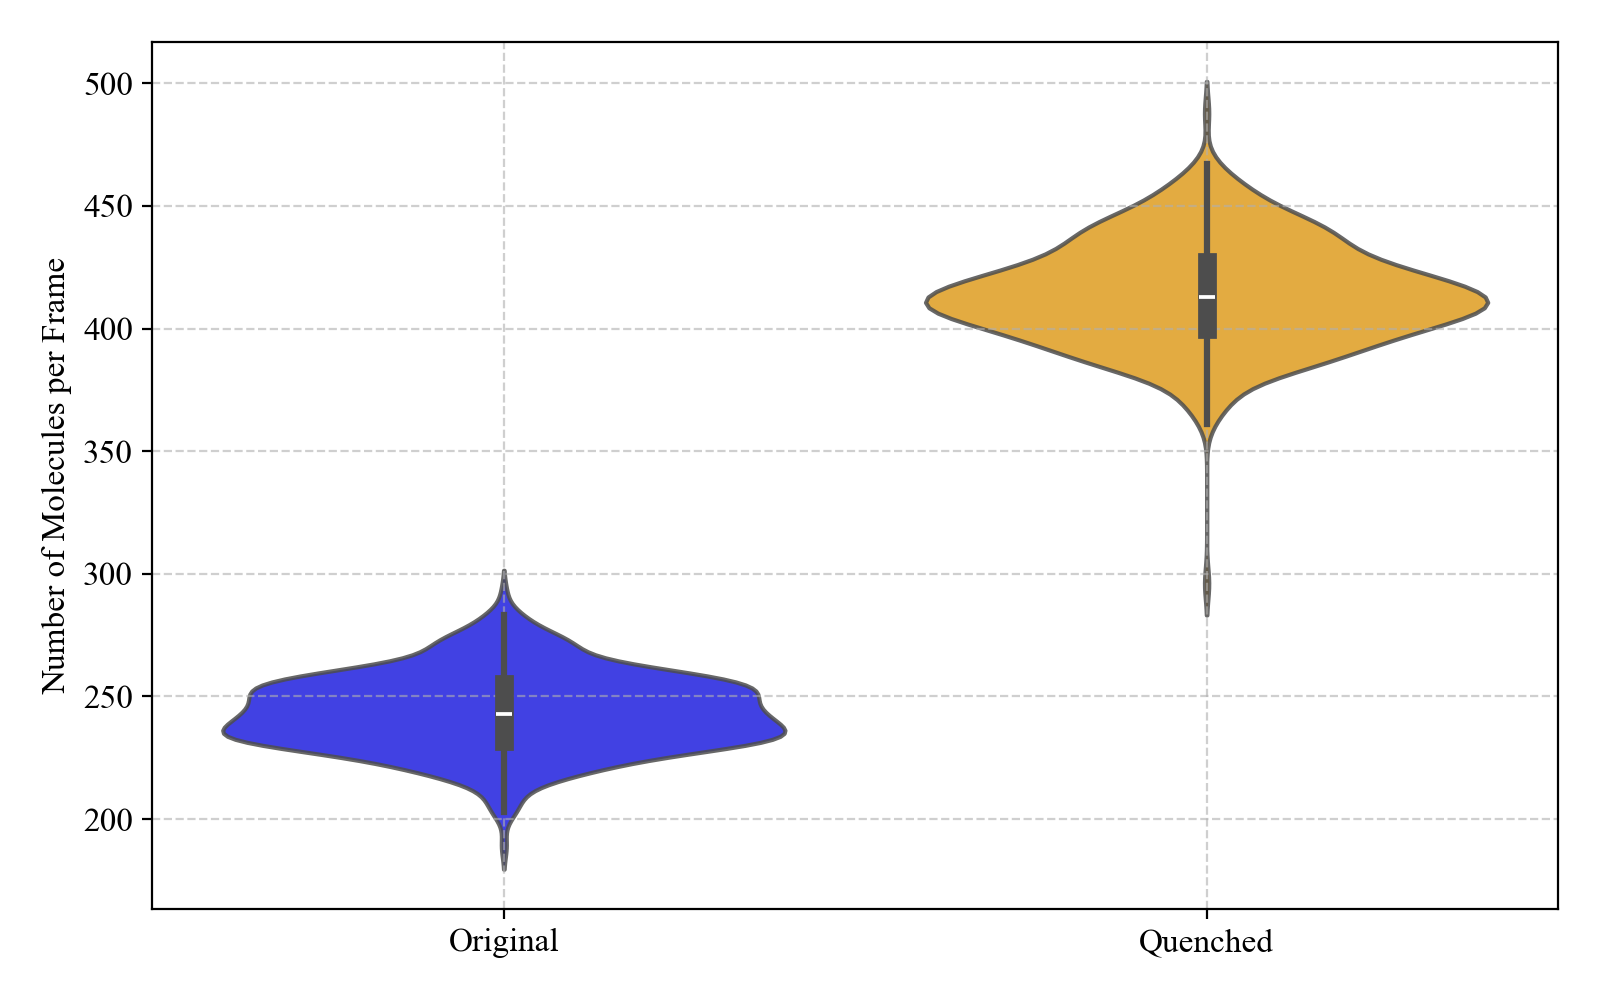
\includegraphics[width=1\linewidth]{Images/early_earth/new_415_violins.png}
    \caption[Violin plot: Molecules identified in select 415 frames before and after quenching]{Molecules identified in select 415 frames before and after quenching.}
    \label{fig:415_new_violins}
\end{figure}

With the addition of molecular signatures, as described in Section \ref{sec:exploring_new_mol_configs}, we note a new trend in the number of unique formulas after quenching, shown in Figure \ref{fig:415_new_formulas}.

\begin{figure}[!ht]
    \centering
    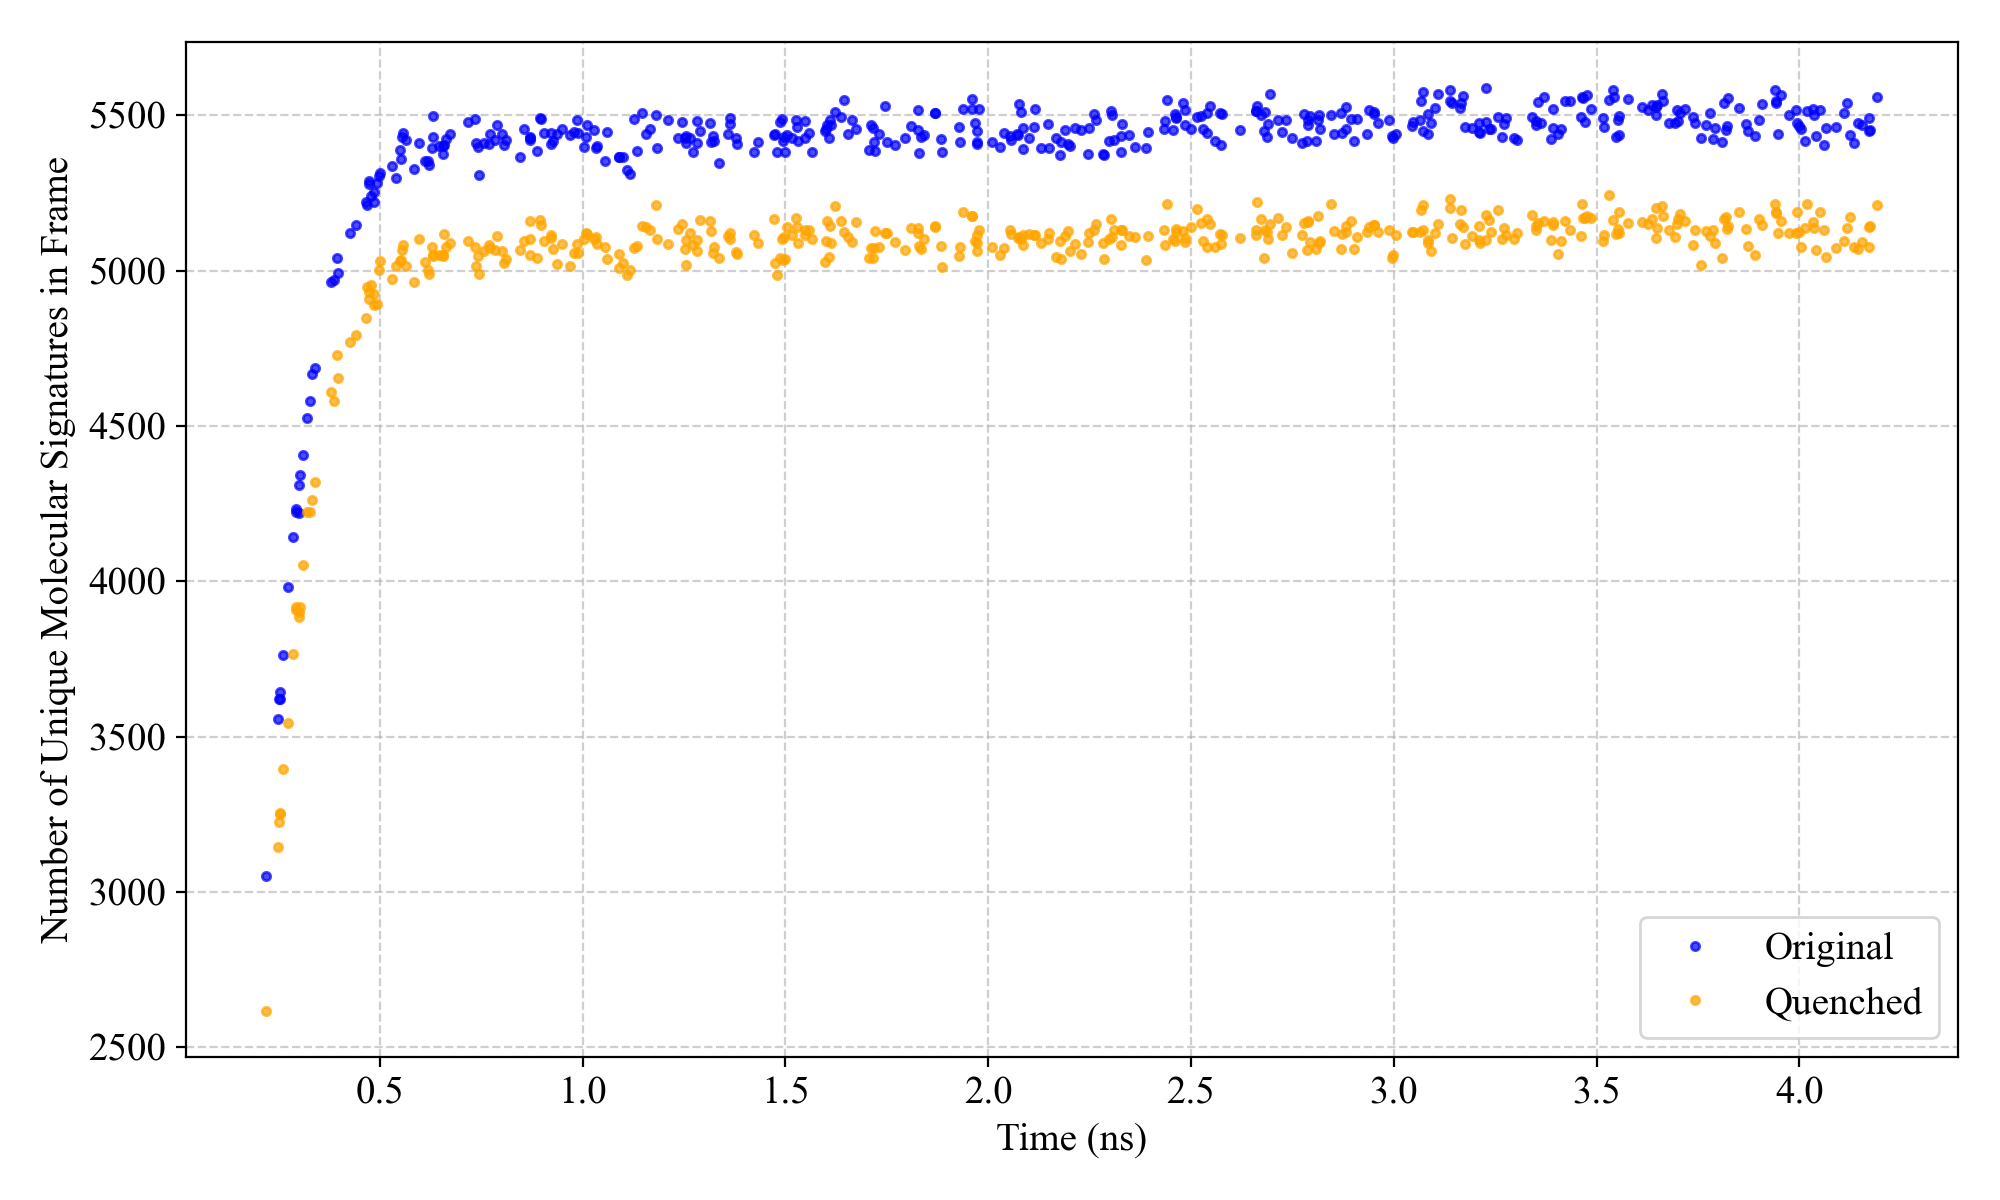
\includegraphics[width=1\linewidth]{Images/early_earth/new_415_quench_formula_vs_frame.png}
    \caption[Unique fragment signatures before and after quenching]{Number of unique fragment signatures before and after quenching 415 select frames from 2500 K to 300 K.}
    \label{fig:415_new_formulas}
\end{figure}

Unlike the first analysis, where the total number of formulas in a frame increased slightly after quenching, we see that the number of unique molecular signatures decreases when each frame is quenched.
This further supports the hypothesis that fragments aggregate into larger, more chemically complex molecules as the temperature drops.

\section{Discussion of Results}
\label{sec:hero_run_interpretation}

Large-scale reactive simulations like the Early Earth Hero Run provide an opportunity to explore the synthesis of prebiotic molecules under plausible early Earth conditions.
This run represents one of the largest reactive molecular dynamics simulations ever conducted with a machine-learned potential. 
After refining the distributed data analysis pipelines used in characterizing the synthesized products and defining new molecules of interest, we note significant improvements to the accuracy and efficiency of structure detection.
Further, the assignment of molecular connectivity signatures to each fragment allows for a more granular view of the diversity of molecular configurations produced throughout the simulation.

The trajectory data produced by this massive Hero Run simulation stands to be a practical source of molecular configurations that could be used to refine the ANI training datasets.
The small and medium Early Earth systems showed new configurations being sampled, but nowhere near the diversity and complexity shown by the Hero Run.
Throughout the simulation, many large molecules are sampled that go uncharacterized by \verb|df_molecule|, where names are assigned to molecules of interest. 
Figure \ref{fig:largest_mol_vs_time} plots the largest molecular fragment at every time step in the simulation.

\begin{figure}[!ht]
    \centering
    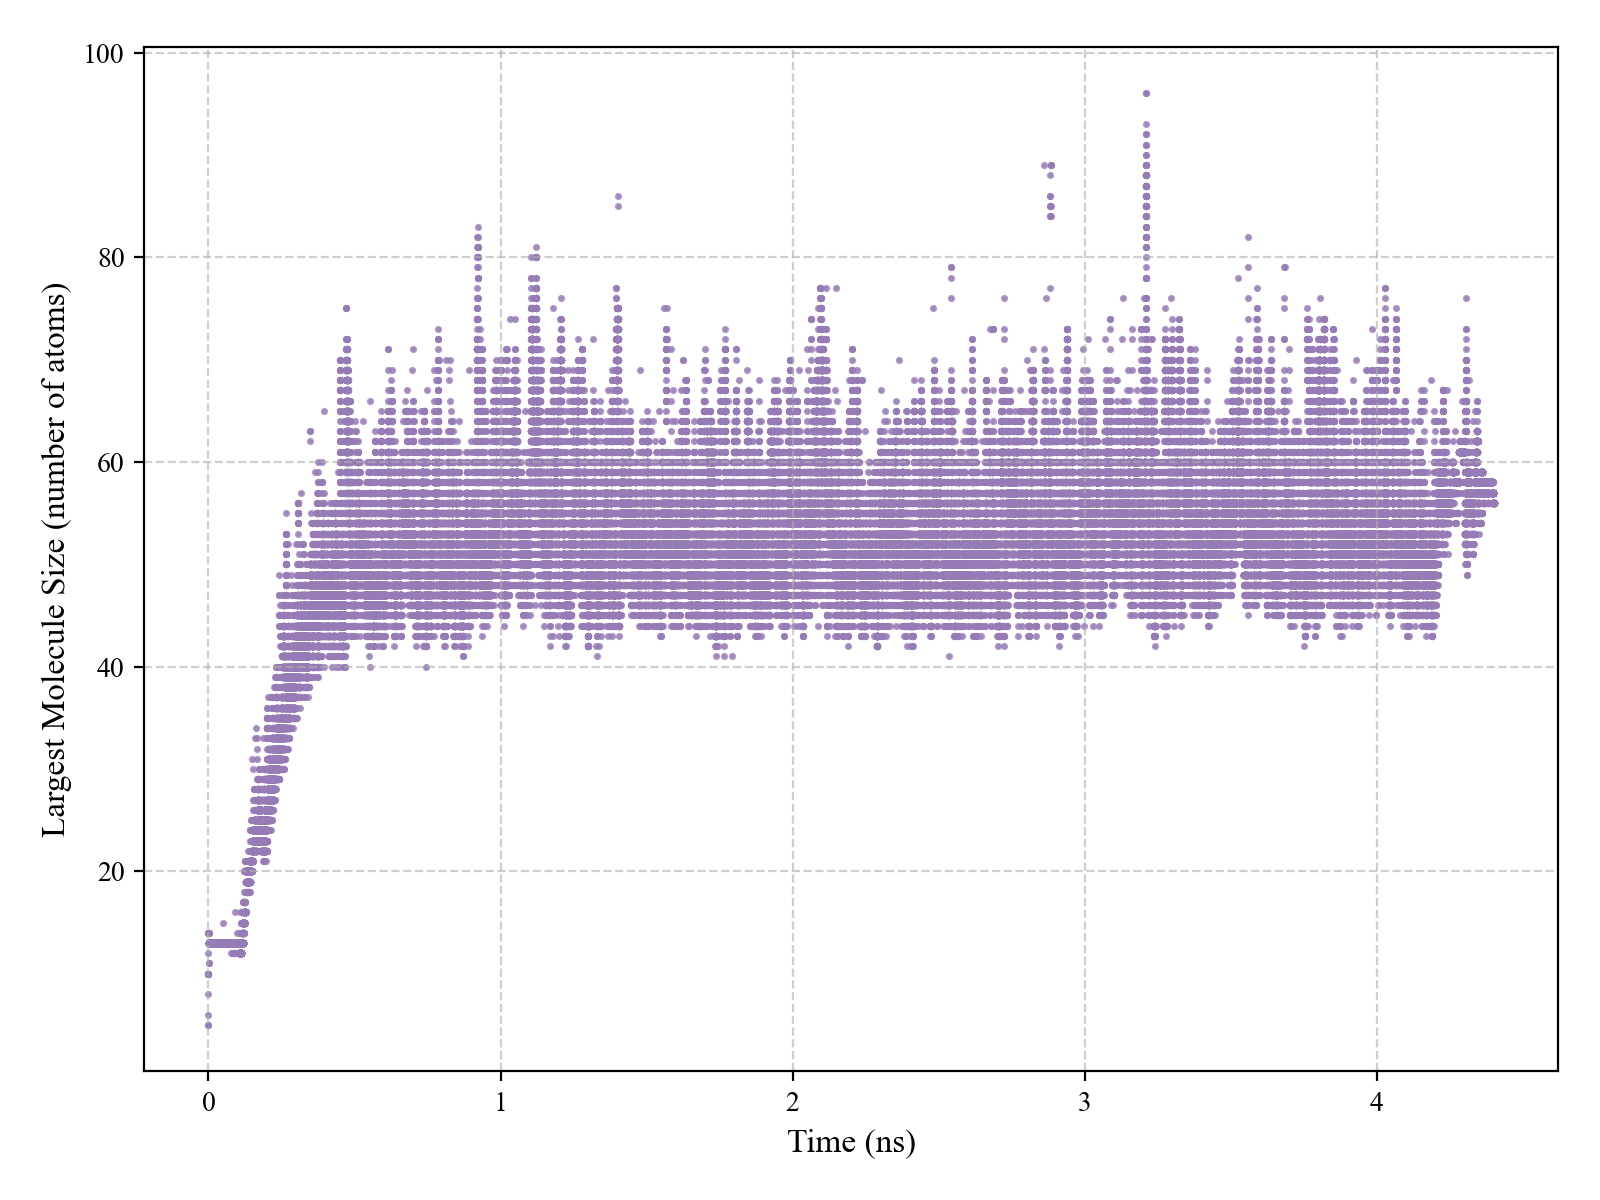
\includegraphics[width=1\linewidth]{Images/early_earth/updated_largest_mol_vs_time.png}
    \caption[Largest molecule per frame throughout the Hero Run simulation]{The number of atoms in the largest molecular fragment in each frame versus time.}
    \label{fig:largest_mol_vs_time}
\end{figure}

A key observation from this data is the emergence of a 96-atom molecule at 3.21 ns, shown in Figure \ref{fig:largest_mol}, the largest molecular fragment formed throughout the simulation.
This large conformation is difficult to capture in a single screenshot but, out of 96 atoms, the molecule has only one valence violation: an excess bond on a nitrogen.
The presence of a double bond between nitrogen and carbon was inferred by \verb|OpenBabel| \cite{babel} when generating a connectivity, and this can be easily fixed by sanitizing the structure with \verb|RDKit|.
The SMILES for this structure was generated using \verb|RDKit| was used to visualize the 2D structure in Figure \ref{fig:largest_mol}(B).
This SMILES yields no search results in PubChem \cite{pubchem}, and this is only one of many likely novel structures produced by this simulation.

\begin{flushleft}
\begin{multiFigure}
    \addFigure{0.532}{Images/early_earth/largest_mol.png}
    \addFigure{0.468}{Images/early_earth/96_atom_2d.png}
\captionof{figure}[Largest molecule synthesized in the Hero Run simulation]{The largest molecule ($N=$ 96 atoms) formed throughout the Hero Run. Identified at frame 256,780, 3.21 ns into the simulation.}
\label{fig:largest_mol}
\end{multiFigure}
\end{flushleft}

The emergence of this molecule, especially given the fact that it is chemically viable, speaks to the reliability of predicted potential energy surfaces by ANI models, capable of enabling stochastic exploration of highly diverse molecular configurations.
The detection of this and other complex molecules is possible due to the development of GPU-accelerated data analysis pipelines, which are necessary to parse over 100 terabytes of trajectory data.
By assigning connectivity signatures and filtering by structural characteristics, we are able to capture nuanced chemical diversity.

Beyond molecular diversity, these results demonstrate the utility of large-scale reactive simulations as a generative source of data.
While large molecular configurations have been shown to be common occurrences under these simulated prebiotic conditions, the vast majority of data is in small molecular fragments.
This provides an excellent route for data-driven model improvement.
Molecules identified here, particularly structures that are uncharacterized by the current ANI ensemble, can serve as high-value candidates for expanding training datasets. 
Utilizing the data produced by this simulation would shift the Hero Run from solely a large-scale simulation, which tests the capabilities of state of the art chemical software and high-performance computing hardware, into a data-mining frontier for active learning applied to model training.
